\documentclass[10pt]{amsart}
\usepackage{palatino}
% The Proposal and Award Policies and Procedures Guide
% (PAPPG: https://www.nsf.gov/publications/pub_summ.jsp?ods_key=pappg)
% mandates, in Chapter 2, section B.2, that the main text should have a font size no less
% than 11 points for *most* typefaces (including Computer Modern Roman and Times (new) Roman).
% 
% Actually, Helvetica (a.k.a. Arial), Palatino and Courier New can drop
% to 10 point font size, according to the PAPPG,  but be aware:
% 10-point fonts (whatever the typeface) will promote reader fatigue.
% Reader fatigue never works to the author's advantage.
%
% This sample is set in 12 point type.
%
\usepackage{amsmath,amsthm,amssymb,amscd}
\usepackage{graphicx}
\graphicspath{{figures/}}
\usepackage{subcaption}
\usepackage{epsf}
\usepackage{cite}		% compress citations
\pagenumbering{gobble}		% Research.gov wants no page numbering
\tolerance9000
%
% The Proposal and Award Policies and Procedures Guide
% (PAPPG: https://www.nsf.gov/publications/pub_summ.jsp?ods_key=pappg)
% mandates, in Chapter 2, section B.2, that margins must be at least 1 inch in all directions.
%
\advance\paperheight1.00cm
\advance\textheight1.00cm
\advance\vsize1.00cm
\advance\topskip-0.5cm
\advance\voffset-0.5cm
%
\oddsidemargin0.15cm
\evensidemargin0.15cm
\textwidth16.1cm
%
%
\renewcommand{\footnotesize}{\small\spaceskip4pt plus1.5pt}
%
\newtheorem{thm}{Theorem}[section]
\newtheorem{prop}[thm]{Proposition}
\newtheorem{cor}[thm]{Corollary}
\newtheorem{lemma}[thm]{Lemma}
\theoremstyle{definition}
\newtheorem{notn}[thm]{Notation}
\numberwithin{equation}{section}

\newcommand\Z{{\mathbb Z}}
\newcommand\Q{{\mathbb Q}}
\newcommand\R{{\mathbb R}}
\newcommand\C{{\mathbb C}}
\newcommand\F{{\mathbb F}}
\newcommand{\G}{{\mathcal{G}}}
\newcommand{\T}{{\mathcal{T}}}
\newcommand\Hom{\text{Hom}}
\newcommand\rank{\mathop{\text{rank}}}
\let\tensor=\otimes

\begin{document}

\centerline{\bf \Large Project Summary}
\setcounter{section}{0}
\vskip 1.0\linespacing 

Radio-frequency (RF) phased-array systems optimized with machine learning have become powerful tools in science and engineering, with applications in particle astrophysics \cite{Vieregg_2016,AVVA201746,electronics10040415,Aguilar_2021}, polar research \cite{arnold_2020,9670670}, and 5G mobile \cite{5G_review_paper}.  Phased-arrays are comprised of RF antennas working in tandem to boost received signal sensitivity, and to actively scan transmitted signals without moving parts.  Two pathways for progress in phased array design and production that will enhance future scientific work are cost reduction and the use of open-source software.  The electromagnetic response of phased arrays are designed with expensive, proprietary software that does not interface with open-source machine learning tools \cite{10.3390/electronics8121506}.  They are then manufactured using costly and time-consuming traditional machining techniques.  Ongoing scientific and engineering efforts can be enhanced by a solution that allows machine learning to flourish, reduces design and manufacturing costs, and diversifies participation by reducing financial barriers.  Such a solution can enhance STEM education with computational electromagnetism, machine learning, and 3D printing by integrating these topics into the curriculum.

We propose to create the first open-source CEM and additive manufacturing ecosystem capable of 3D-printing phased arrays with conductive filament \cite{10.3390/electronics8121506, yurduseven,8786183}.  We have already shown that open-source CEM tools used in photonics can drive the RF phased-array design process \cite{electronics10040415,meepcon2022,10.1016/j.cpc.2009.11.008}.  This research will support diverse projects like IceCube Gen2 (radio), Center for Remote Sensing and Systems (CReSIS) missions, and Office of Naval Research (ONR) radar projects.  One application in particle astrophysics is the Askaryan Radio Array (ARA), in which phased arrays have increased sensitivity to ultra high-energy neutrino (UHE-$\nu$) interactions in the ice sheet beneath the South Pole \cite{PhysRevD.105.122006}.  The arrays are vertically polarized, due to mechanical constraints within the ice.  By combining machine learning with CEM, we seek a \textit{horizontally polarized} design that overcomes these mechanical constraints, boosting the chances of making the first UHE-$\nu$ observations in history.  This research will \textit{accelerate} and \textit{diversify} research in UHE-$\nu$, climate science, and RF engineering by \textit{translating} successes in CEM and materials research.  This work will be integrated into our curriculum and research programming at Whittier College, officially a Hispanic Serving Institution (HSI).  This work touches upon three of the 10 Big Ideas from NSF: Windows on the Universe, NSF INCLUDES, and Navigating the New Arctic.

This work will provide research and educational opportunities to diverse undergraduates at Whittier College.  We have a proud tradition of providing access to higher education to Spanish-speaking and historically marginalized students, and we are the only HSI member of the IceCube Gen2 collaboration.  People of color and first-generation students make up 63\% and 29\% of our student body, respectively.  Internal assessment studies indicate that students of color receive lower grades than their peers in introductory STEM courses.  We have learned from workshops hosted by the Cottrell Scholars Network that emphasizing the dignity and self-efficacy of diverse students can increase their performance \cite{cottrell1,cottrell2}.  Emphasis in these areas makes students feel they \textit{belong} in our courses, despite encountering adversity. In keeping with the theme of \textit{translation}, and in order to emphasize the dignity of our students no matter their background, we seek to create a bilingual (Spanish and English) mobile application (app) that introduces STEM concepts within a welcoming digital environment.

There is precedent for learning apps enhanced by machine learning in the Duolingo method for language and mathematics \cite{duolingo_whitepaper}. We seek to provide data insights about student learning to instructors through the app, which will lead to more efficient and customized classroom instruction.  A prototype application is being built by Whittier College undergraduates.  The creation and implementation of this program represents an opportunity for Whittier College students to enhance the learning experience for their peers while gaining valuable coding and machine learning experience.  In addition to algorithms presented within the Duolingo method, the educational data mining (EDM) literature provides examples of apps that boost engagement and success in introductory STEM courses \cite{edm1,edm2,edm3,edm4}.  Members of our community have shared that translating mathematics and physics exercises into Spanish aids in solving them.  Our application will boost their skills and build confidence by offering them engaging, game-like physics training in the language of their choice.  Finally, we propose to create a bilingual lecture series and recruitment events designed to welcome the broader community into the Whittier College environment.

\clearpage

\centerline{\bf \Large Project Description: Intellectual Merits}
\setcounter{section}{0}
\vskip 1.0\linespacing

\label{sec:top}

Radio-frequency (RF) phased arrays have applications in radar telemetry, 5G telecommunications, ground-penetrating radar (GPR), scientific instrumentation, and remote sensing \cite{Vieregg_2016,AVVA201746,arnold_2020,PhysRevD.105.122006,10.3390/s21186091,10.1016/j.jappgeo.2022.104876,phased_array_book}.  In the one-dimensional case, $N$ three-dimensional RF antennas are arranged in a line with fixed spacing.  In the two-dimensional case, $N \times M$ three-dimensional antenna elements are arranged in a two-dimensional grid with fixed spacing in both dimensions.  The signal to noise ratio (SNR) of received signals in arrays of dimension $N$ is boosted by a factor of $\approx \sqrt{N}$, because the $N$ signals are combined coherently while thermal background noise adds like $\sqrt{N}$ \cite{AVVA201746}.  The SNR boost is critical for scientific observations.  For example, systems created at the Center for Remote Sensing and Integrated Systems (CReSIS) are flown in polar regions to perform radar sounding of ice sheets for the purposes of geophysics and climate science \cite{arnold_2020}.  Reflected signals carry information about glacial depth, temperature, and internal structure.  

Traditionally, RF phased arrays are designed with commerical computational electromagnetism (CEM) software.  Radio antennas and phased arrays have \textit{radiation patterns} that define directions of maximum transmission power and received sensitivity.  Radiation patterns have a main lobe in which most of the radiation is concentrated, and the angular width of the main lobe is called the beam width.  The S-parameters quantify the system efficiency.  CEM packages like XFDTD are used to model radiation patterns and S-parameters as a function of frequency.  The XFDTD package, for example, relies on the finite difference time domain (FDTD) method. The FDTD approach is a CEM technique in which spacetime and Maxwell’s equations are discretized.  The cost of these products ranges between \$5,000 and \$40,000 USD.  These costs are prohibitive for HSI undergraduate institutions like Whittier College.  Removing financial barriers will allow diverse undergraduates to study professional RF design. 

Another drawback of commercial CEM software is the lack of source code access impedes the incorporation of modern machine learning packages.  Phased array properties are determined by the shape of the RF elements and the grid properties of the array.  The parameter space is driven by the complex variety of RF element shapes.  When combined with open-source CEM software, modern machine learning algorithms can locate optimal solutions.  The authors of \cite{10.3390/electronics8121506} review a number of open-source CEM packages.  One interesting choice they describe is the MIT Electromagnetic Equation Propagation (MEEP) package \cite{10.1016/j.cpc.2009.11.008}.  Though MEEP was designed for $\mu$m wavelengths in photonics applications, we have shown that the scale-invariance of Maxwell's equations allows MEEP users to translate designs to wavelengths at the cm-scale.  We have also shown that MEEP can drive the RF phased-array design loop, and that 3D printer schematics can be extracted from this process \cite{electronics10040415,meepcon2022,10.1016/j.cpc.2009.11.008}.  Our proposal will allow diverse students to experience translating machine learning results into tangible solutions.  

Filament for 3D printers that is conductive in the RF bandwidth is now available commercially.  Funded through an NSF Translational Impact (TI) award (1721644), Multi3D LLC. has produced filament with a resistivity of just $10^{-2} \Omega$ cm: the Electrifi filament.  Several antenna designs have already been produced \cite{8786183,10.1049/iet-map.2017.0104}.  The measured properties match commercial CEM software output.  There are, however, virtually no examples of 3D printed RF phased arrays in the [0.1 - 1] GHz bandwidth.  This bandwidth is the most relevant for the aforementioned applications in particle astrophysics (UHE-$\nu$) and geophysics.  Further, whole new designs can be discovered that improve on common designs by merging machine learning packages with MEEP.  In Sec. \ref{sec:cem}, we review progress already made at Whittier College.  In Sec. \ref{sec:askaryan}, we show how this work enhances the field of UHE-$\nu$ detection.  In Sec. \ref{sec:cresis}, we show how this work enhances the field of radio glaciology.  In Sec. \ref{sec:int}, we articulate our vision for the integration of this research into our STEM curriculum.  In Sec. \ref{sec:broad}, we describe the phase of this project designed to help us provide a better education to our students and broader community.  In Sec. \ref{sec:time_im}, we share project planning analysis that including measurable goals and a detailed work timeline.

\section{Computational Electromagnetism and Additive Manufacturing}
\label{sec:cem}

In Summer 2020, we received a Faculty Fellowship from the Office of Naval Research (ONR) to design phased arrays in the [0.1 - 5] GHz bandwidth.  This bandwidth is relevant for projects like IceCube Gen2 (radio)\footnote{Whittier College is a member institution of the IceCube Gen2 collaboration that seeks to detect UHE-$\nu$.}.  Given our background in RF detectors for UHE-$\nu$ observations in Antarctica (see Sec. \ref{sec:askaryan}), we were qualified to introduce RF phased arrays to our Navy colleagues.  The audience included engineers and programmers that work in acquisition and development for the Naval Surface Warfare Center (NSWC), Corona Division (NSWC Corona).  Our goal was to design a phased array transmitter integrated within an anechoic chamber to mimic moving radar echoes.  The facility will serve as a testing facility for active radar systems.  We began by giving lectures on the electromagnetism of phased arrays, with scientific applications.  To minimize costs and increase undergraduate access, we decided to investigate open-source CEM tools. 

%\begin{figure}
%\centering
%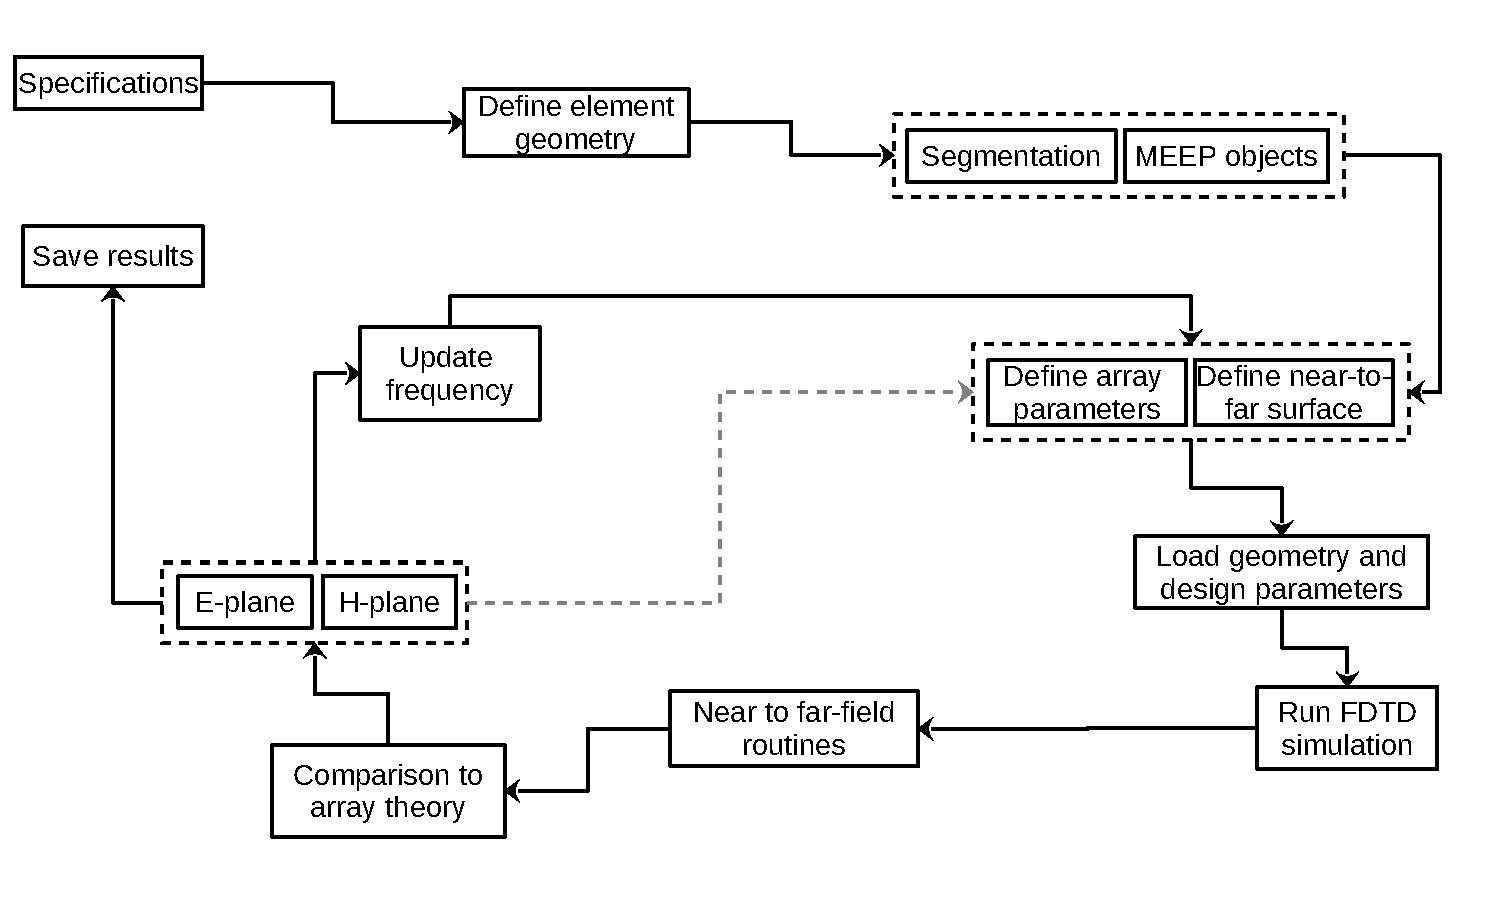
\includegraphics[width=0.85\textwidth]{diagram3.pdf}
%\caption{\label{fig:design}  Our design process for RF phased arrays from \cite{electronics10040415}, adapted from Fig. 1 of the review \cite{10.3390/electronics8121506}.}
%\end{figure}

We encountered the aforementioned review article covering open-source CEM tools in the open-access journal \textit{Electronics}.  Our design flow was adapted from the review to include specific tasks required for phased arrays, and algorithms for the computation of far-field radiation patterns.  MEEP was noted by the authors in the review as the most advanced among open-source FDTD programs, but they did not benchmark it against commercial CEM tools due to the ``steep'' learning curve.  In Summer 2020, we ascended the learning curve and adapted MEEP to RF systems.  A key insight was that MEEP takes advantage of the \textit{scale invariance} of Maxwell's Equations.  The simplest way to understand this is to understand how MEEP uses relative units when discretizing Maxwell's equations. 

Like other FDTD methods, MEEP uses a Yee lattice to discretize Maxwell's equations \cite{10.1109/tap.1966.1138693}.  When the speed of light is set to unity ($c = 1$), lattice distance and time units become the same.  Frequency and wavelength units are the inverse of each other.  But distance and wavelength can take \textit{any} unit of length in the Yee lattice.  Most MEEP users interpret this unit as 1$\mu$m.  For example, a \textit{relative} frequency (unit-less) of 0.5 corresponds to a \textit{relative} wavelength of 2.  When interpreted as 2 $\mu$m, the frequency is 150 THz in real units in the optical bandwidth.  Interpreted as 2 cm, the real frequency is 15 GHz.  A \textit{relative} frequency of 0.05 corresponds to the RF frequency 1.5 GHz.  Assuming components have good RF conductivity, we have re-purposed MEEP as an open-source RF design package.  

\begin{figure}[ht]
\centering
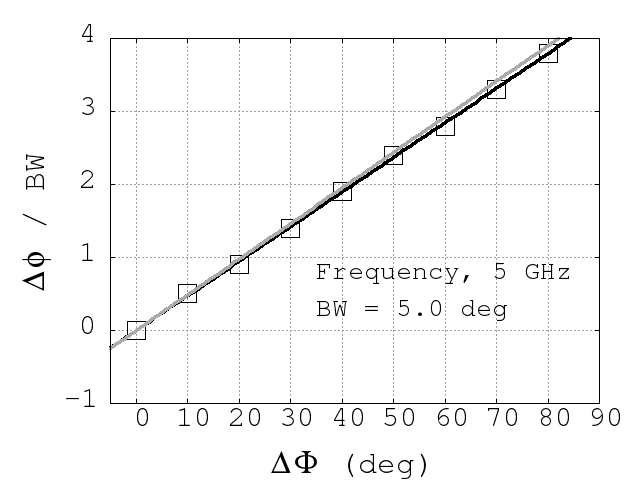
\includegraphics[width=0.33\textwidth]{figures/Oct30_plot1.png}
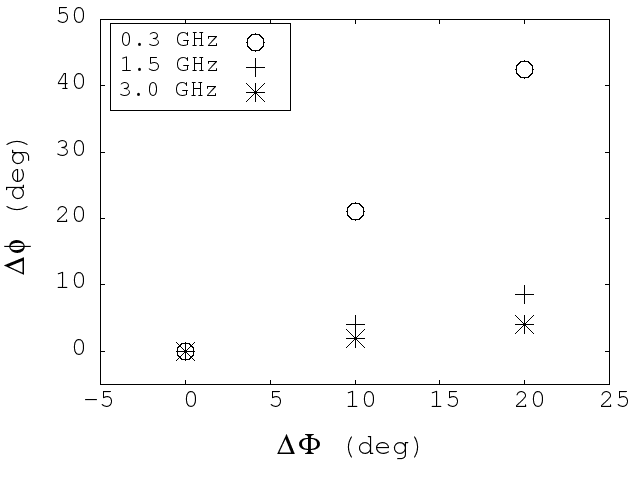
\includegraphics[width=0.33\textwidth]{figures/Aug11_plot2.png}
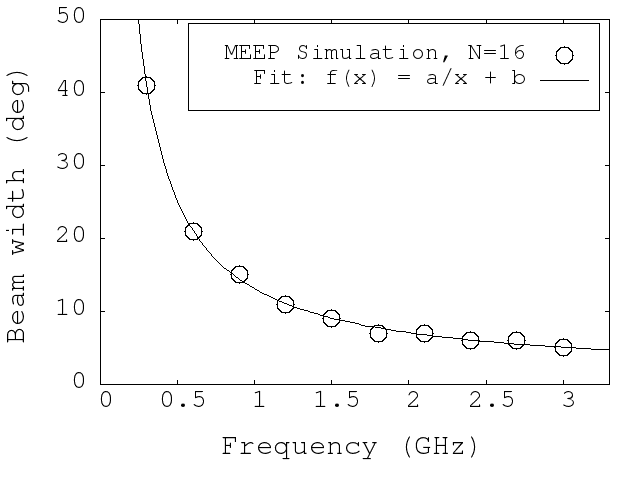
\includegraphics[width=0.33\textwidth]{figures/Aug11_plot1.png}
\caption{\label{fig:pa_1} (Left) The beam angle $\Delta \phi$ divided by the beam width $BW$ for the $N = 16$ one-dimensional Yagi array versus $\Delta \Phi$, the phase shift per element, in degrees. The gray line represents theoretical expectation, and the black line is a linear fit to the data.  (Middle) $\Delta \phi$ versus $\Delta \Phi$ for the $N=16$ version of the one-dimensional horn array, for three frequencies.  (Right) The dependence of the beam width on frequency for the one-dimensional $N=16$ horn array.  The black line is a functional fit to the data $f(x) = a/x + b$ with $a=12.0\pm 0.1$ degree GHz, and $b=1.1\pm 0.2$ degrees.}
\end{figure}

By Fall 2020, we were producing CEM models using MEEP that matched expected phased array properties.  For a one-dimensional array with $N$ elements, there is a linear relationship between the radiated plane-wave direction $\Delta \phi$, and the phase shift per element $\Delta \Phi$.  The $\Delta \phi$ is also called the \textit{beam angle}.  Figure \ref{fig:pa_1} contains results for our first phased array models in which the elements were Yagi-Uda antennas and horn antennas.  The linear relationship between $\Delta \phi$ and $\Delta \Phi$ is evident in the data.  The $\Delta \phi$ is divided by the beam width (BW) in Fig. \ref{fig:pa_1} (left), and is left in degrees in Fig. \ref{fig:pa_1} (middle).  In Fig. \ref{fig:pa_1} (left), the single-frequency $N=16$ Yagi array can steer a 5 GHz plane wave up to four beam widths to the right or left of the forward direction.  In Fig. \ref{fig:pa_1} (middle), results are shown for an $N=16$ array of horn antennas.  Unlike the Yagi-Uda, the horns are broadband radiators.  Thus, the linear relationship is shown for 0.3, 1.5, and 3.0 GHz.  The beam width is not constant, so $\Delta \phi$ was left in degrees in Fig. \ref{fig:pa_1} (middle).  In Fig. \ref{fig:pa_1} (right), the inverse relationship between beam width and frequency is shown. 

We also compute radiation patterns that match array theory.  The pattern of a phased array can be derived from first principles \cite{electronics10040415}.  The \textit{pattern multiplication theorem} states that the radiation pattern of a phased array of $N$ identical elements will be that of a row of $N$ point sources, multiplied by the radiation pattern of the element.  In Fig. \ref{fig:1dhornresults2} (left and middle), the radiated E-field of a $N=16$ horn array is shown in the E-plane (x-y plane).  The radiation pattern is represented by the blue curve in Fig. \ref{fig:1dhornresults2} (right).  The beam angle of the main lobe is $\Delta \phi = 9$ degrees above the x-axis, matching the theoretical expectation in red.  The red curve corresponds to the formula for a row of $N$ point sources, which has a back lobe at $\Delta \phi = 171$ degrees due to symmetry.  The horn array has no back lobe because the individual horns suppress it, as expected from the pattern multiplication theorem and as observed in Fig. \ref{fig:pa_1} (Left, Middle).  Like the theoretical expectation, the CEM pattern has \textit{side lobes} around the main lobe ($\approx -15$ dB).  We achieved similar results for two-dimensional arrays of Yagi-Uda and horns.  Our revelation that MEEP could be used to design RF phased arrays earned the article Top 10 honors for December 2020 - May 2021 from the editors of \textit{Electronics}. 

\begin{figure}
\centering

\includegraphics[width=5.625cm,angle=90]{figures/fields/colorbar.pdf}
%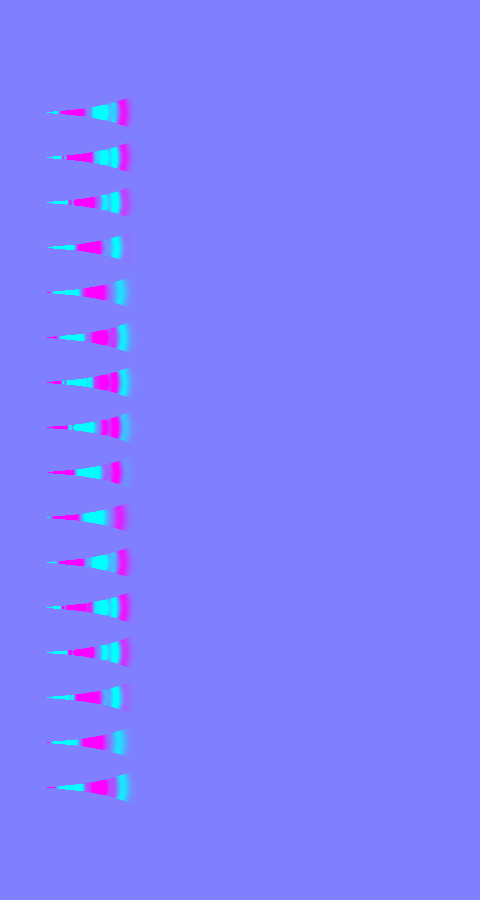
\includegraphics[width=3cm]{figures/fields/ey_phase_horn_t15.png}
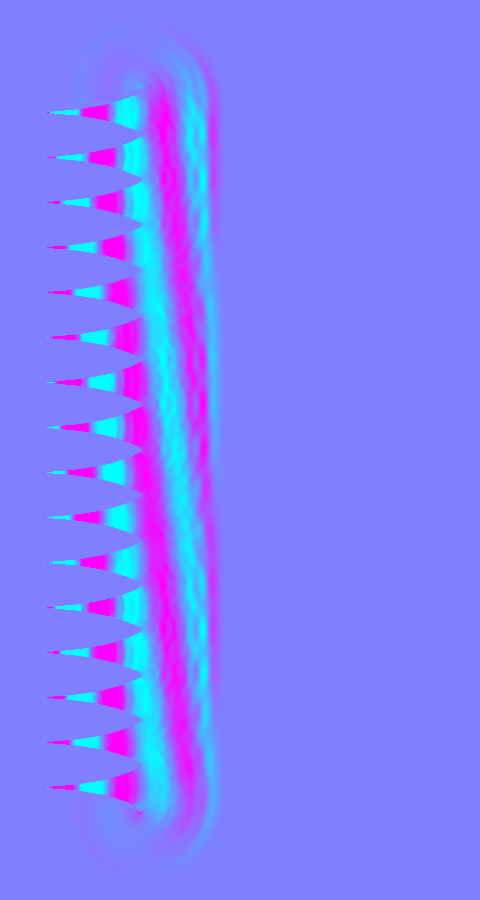
\includegraphics[width=3cm]{figures/fields/ey_phase_horn_t30.png}
%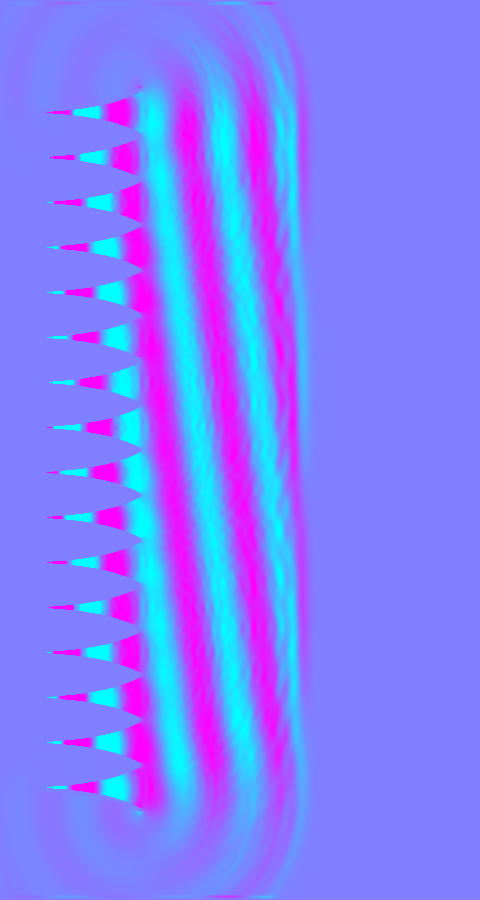
\includegraphics[width=3cm]{figures/fields/ey_phase_horn_t45.png}
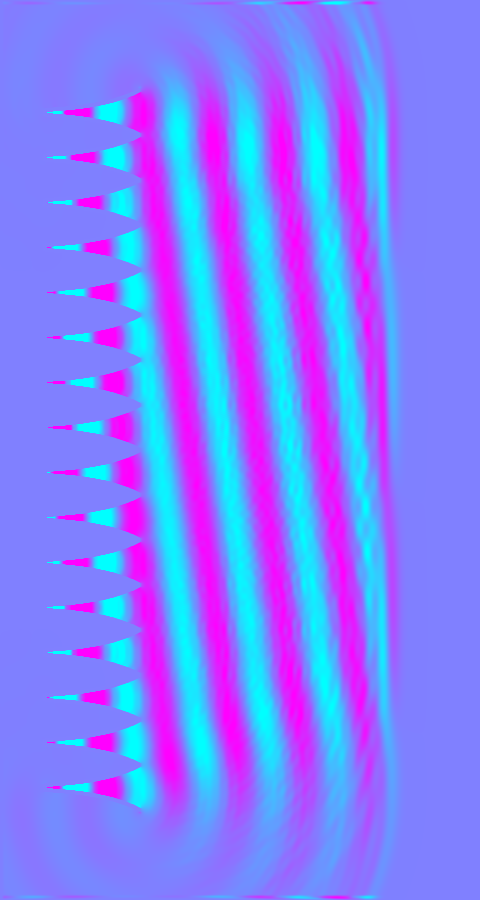
\includegraphics[width=3cm]{figures/fields/ey_phase_horn_t60.png}
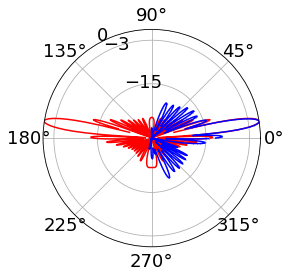
\includegraphics[width=6cm]{figures/fields/rad_patt_field.png}
\caption{\label{fig:1dhornresults2} (Left) The $N = 16$ horn array, radiating the linearly polarized $\vec{E}(x,y,t)$ (y-component shown, in arbitrary units) at $t = 1$ ns into the simulation run, and (middle) at $t = 2$ ns into the run.  The 2D area is $80 \times 150$ cm$^2$.  The frequency is 2.5 GHz, and the beam angle is $\Delta \phi = 9$ degrees above the x-axis. (Right) The normalized radiated power in dB versus $\Delta \phi$ in degrees.  The blue curve represents the results from MEEP, and the red curve is the theoretical expectation from $N$ point sources.}
\end{figure}

\begin{figure}
\centering
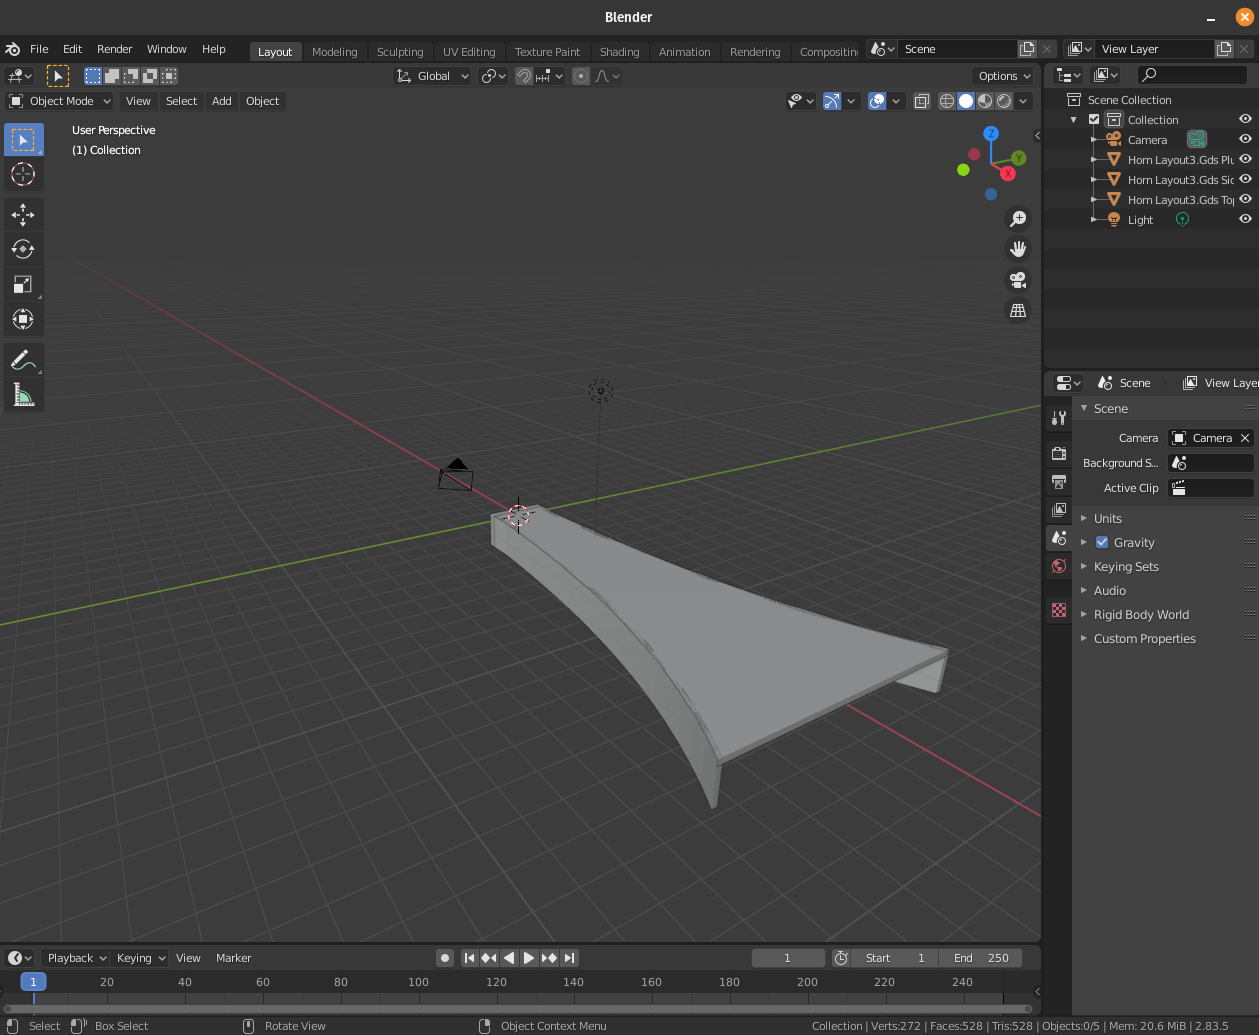
\includegraphics[width=0.4\textwidth]{figures/blender_example.png}
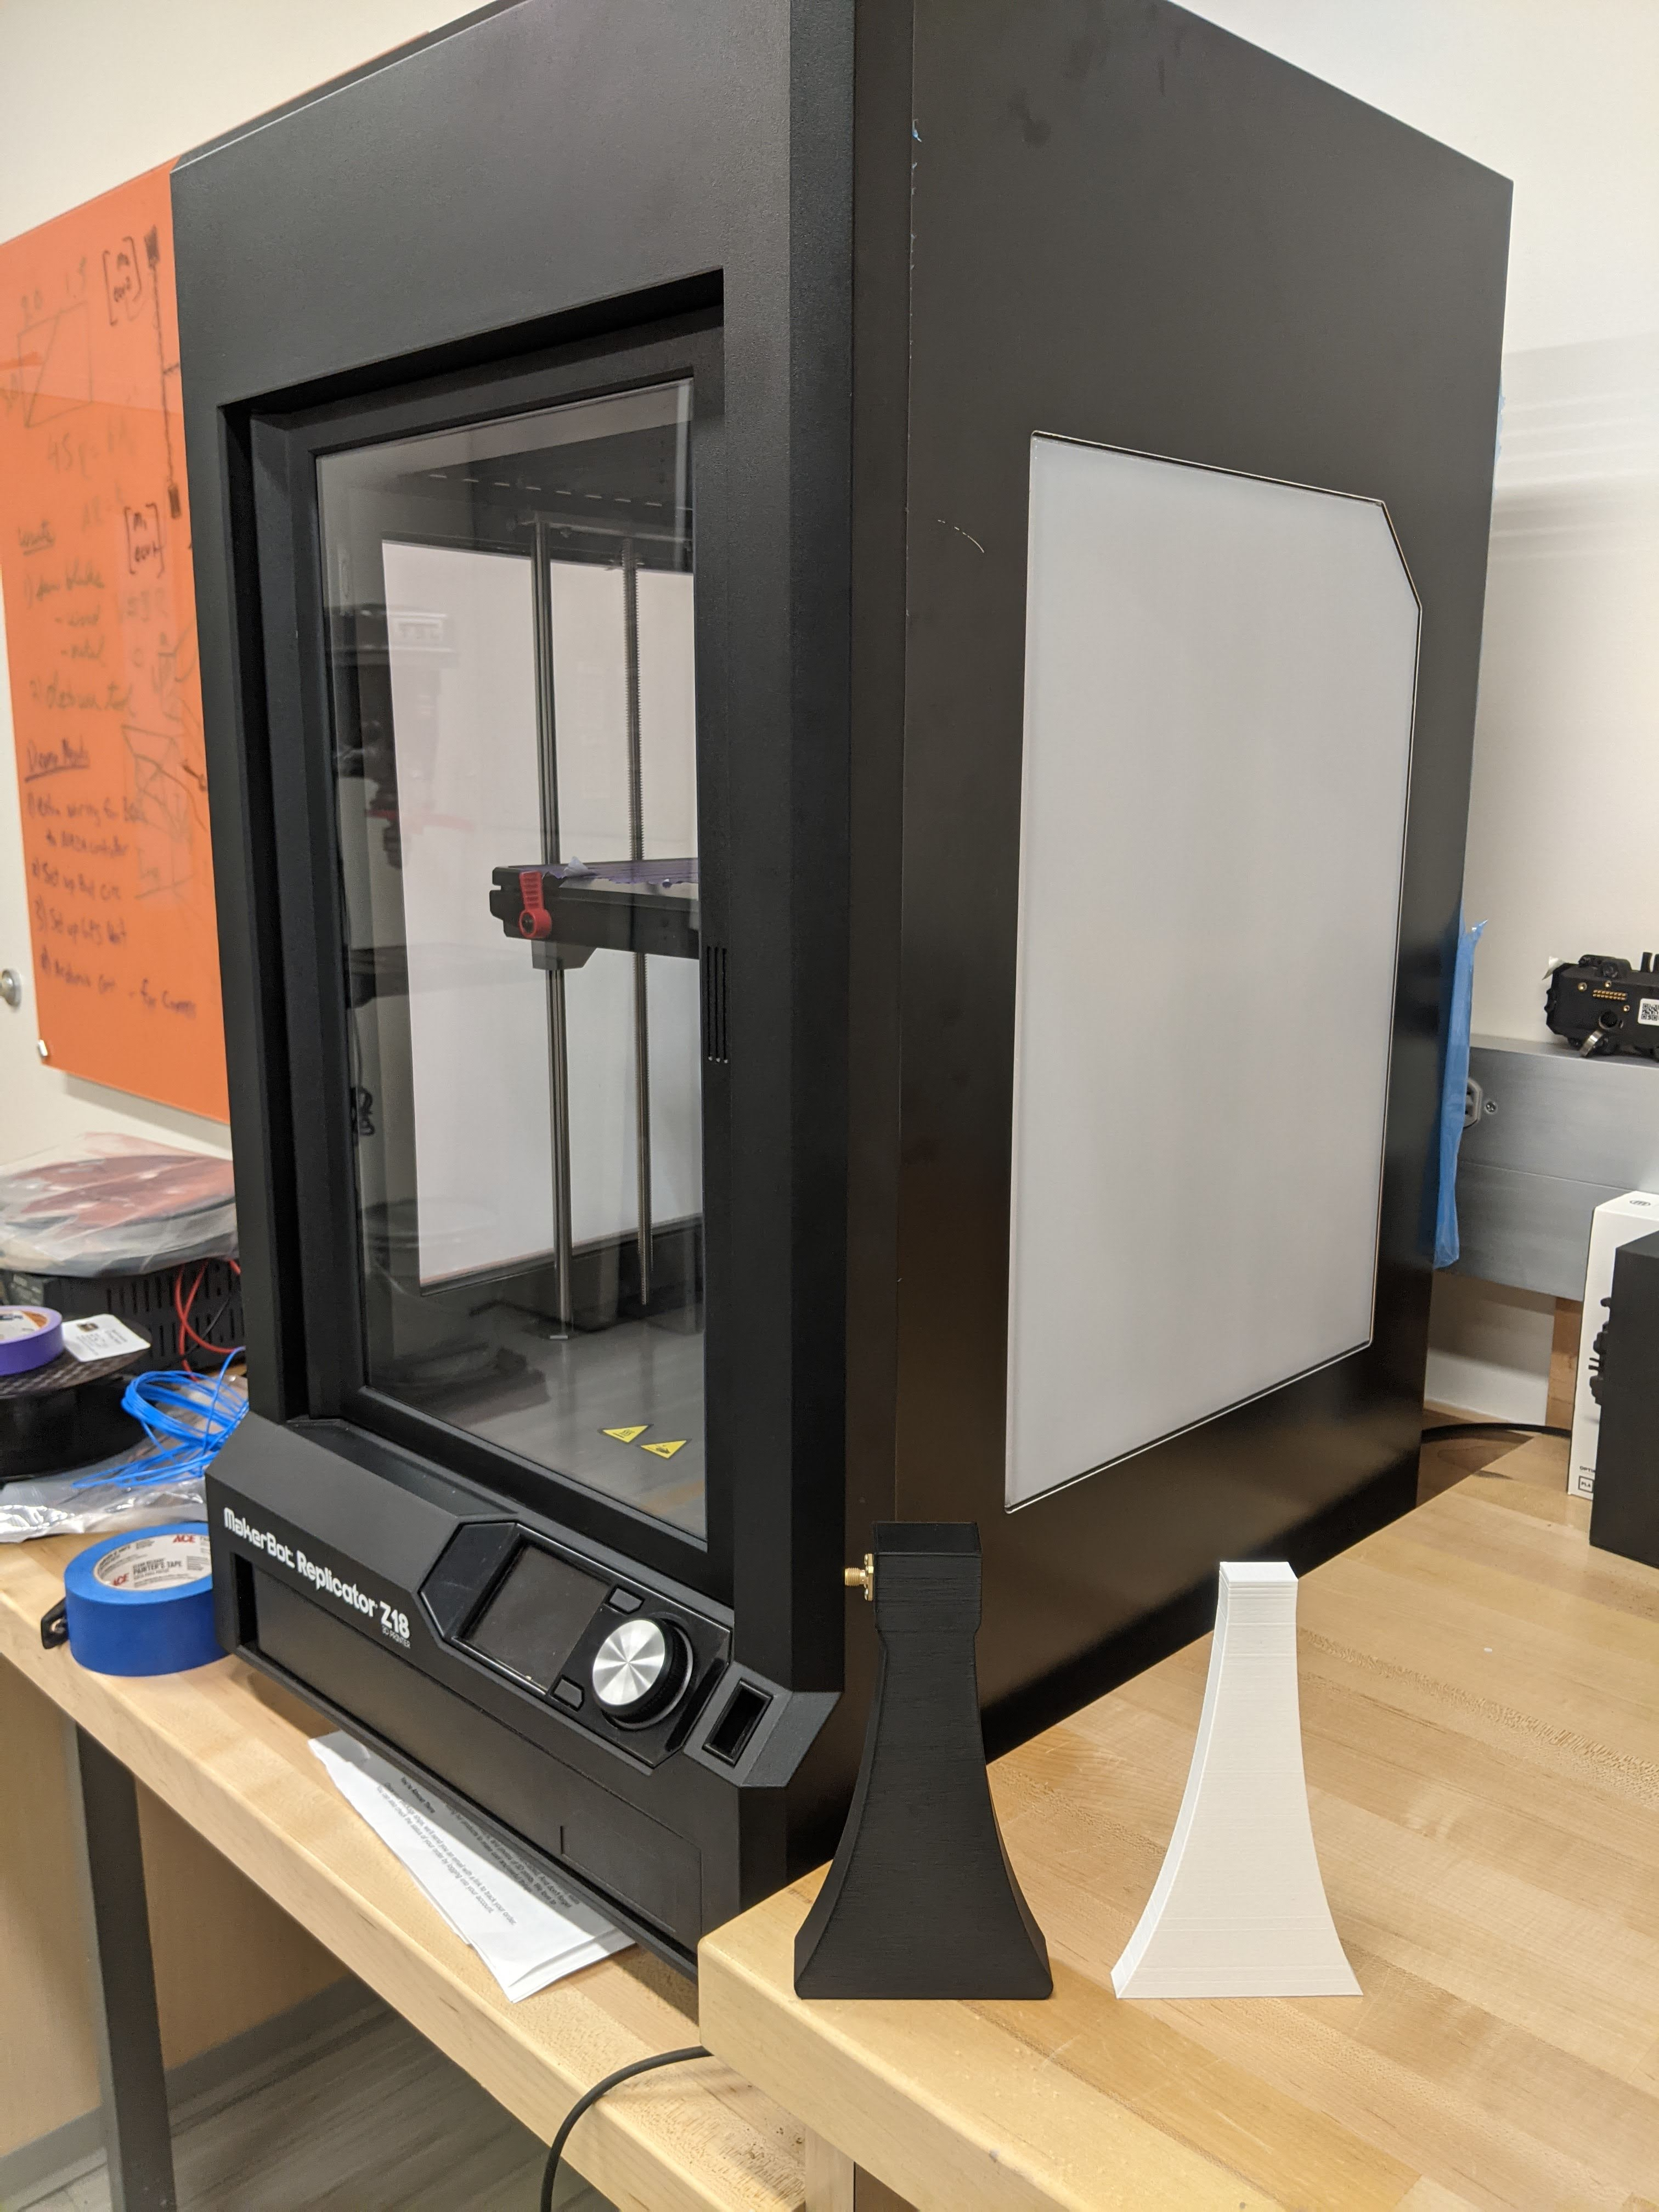
\includegraphics[width=0.25\textwidth]{figures/3dprinter.jpg}
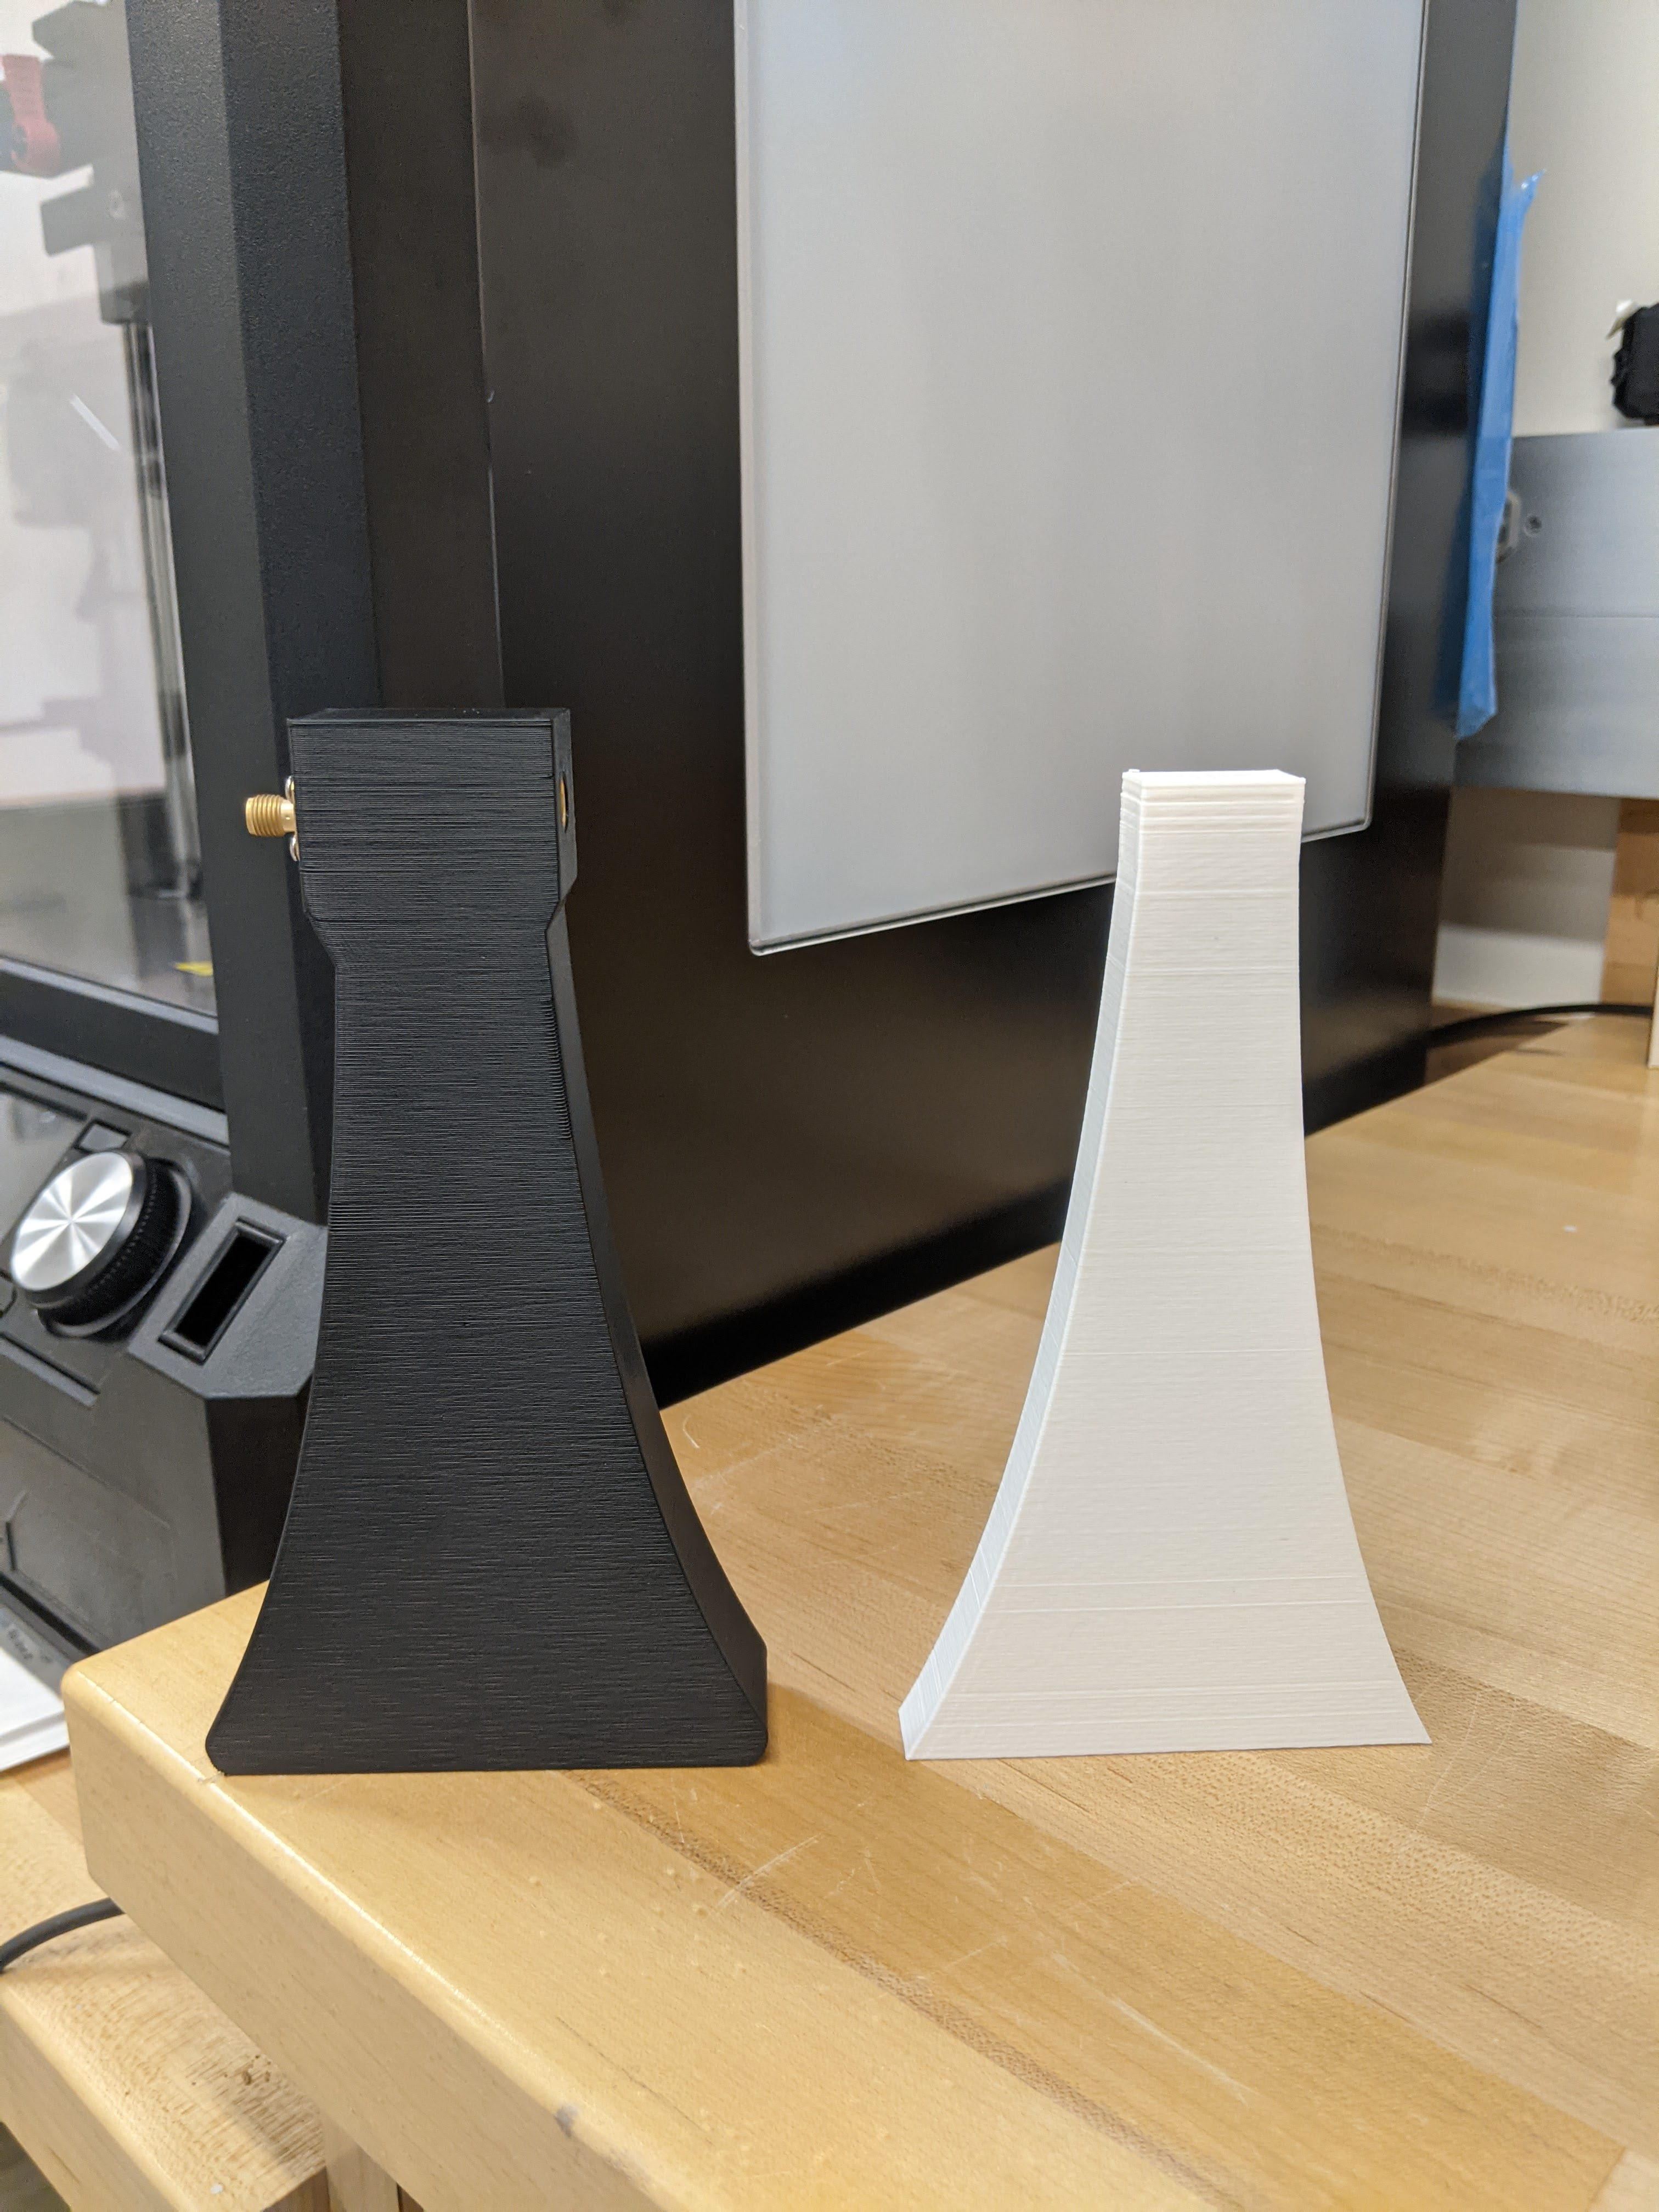
\includegraphics[width=0.25\textwidth]{figures/3dprinter_2.jpg}
\caption{\label{fig:3d_print} (Left) Blender/STL files extracted from MEEP code.  (Middle) MakerBot 3D printer, with PLA horn model (white), and  proto-pasta with SMA connector (black). (Right) Close-up of horns.}
\end{figure}

In Summer 2021, we received a second ONR fellowship to continue the research.  We determined how to integrate open CAD design with MEEP.  As a result, we can now compute the radiation patterns and S-parameters of the exact object we hope to print.  We acquired NinjaTek proto-pasta 3D printer filament, advertised as conductive.  We printed a horn with in-built SMA connecter for RF cables (Fig. \ref{fig:3d_print}).  The proto-pasta result had a measured resistance of $2.5$ k$\Omega$, too large for an RF antenna.  Multi3D LLC, the manufacturer of the Electrifi filament, has now provided resistivity results that compare proto-pasta with Electrifi (Fig. \ref{fig:3d_print2}).  The Electrifi filament will improve resistivity by a factor of 120.  We seek to print new RF antennas, and to measure the radiation pattern and S-parameters. 

\begin{figure}[ht]
\centering
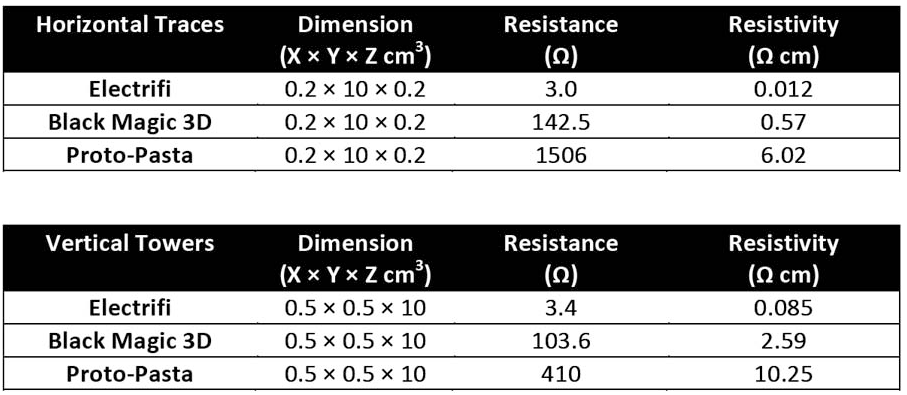
\includegraphics[width=0.85\textwidth,trim=0cm 0cm 0cm 7cm,clip=true]{figures/multi3dllc.png}
\caption{\label{fig:3d_print2} Resistivity results for various 3D printer filaments.}
\end{figure}

In Summer 2022, we received a third ONR fellowship focusing on GPS modernization\footnote{ONR regulations state that a gap year is required for Summer 2023.  For our group, Senior Fellowship eligibility begins in Summer 2024.}.  Alongside this work, we continued to refine the open-source CEM results.  We learned to simulate the full 3D horn element stored in 3D open CAD files using parallel processing, reducing computation time by an order of magnitude.  The results are shown in Fig. \ref{fig:3d_cad}.  In Fig. \ref{fig:3d_cad} (a), the main lobes are designed to point to 0 degrees (x-direction) for the E-plane (x-y plane), and 90 degrees for the H-plane (x-z plane).  The E-plane contains the linearly polarized radiation vector.  In Fig. \ref{fig:3d_cad} (b), the voltage standing wave ratio (VSWR) is shown.  The VSWR is a common figure of merit for RF antennas, related to the S-parameters.  The VSWR approaches 1 for an efficiently radiating antenna, and infinity for no efficiency.  The radiation patterns also match expectations for horn antennas (see Fig. 19 of \cite{8786183}).  The VSWR results demonstrate efficient radiation in the bandwidth [0.5 - 6] GHz.  We presented our progress at the annual MeepCon 2022 at the Massachusetts Institute of Technology (MIT) \cite{meepcon2022}.  We learned new techniques for integrating MEEP and machine learning tools \cite{meepcon2022_2}, and how eager MEEP developers are to collaborate in the RF regime.  

\begin{figure}[ht]
\centering
\begin{subfigure}{0.65\textwidth}
    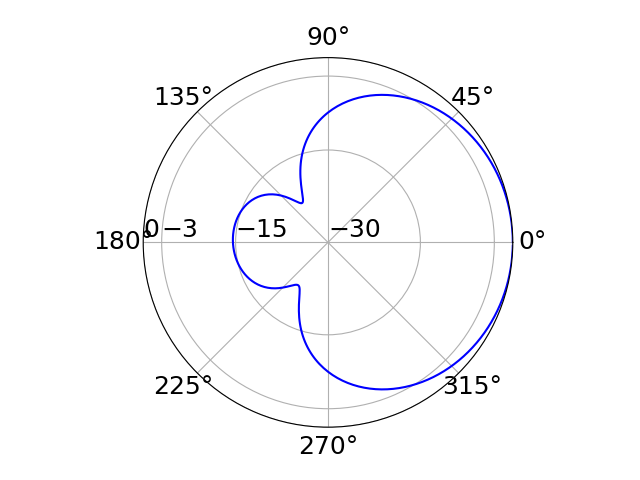
\includegraphics[width=0.49\textwidth]{figures/3DHorn_CAD_0_5GHz_E_plane.png}
	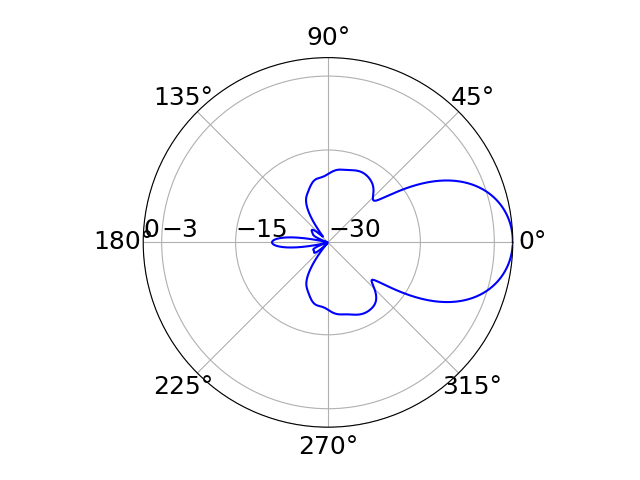
\includegraphics[width=0.49\textwidth]{figures/3DHorn_CAD_5GHz_E_plane.png} \\
	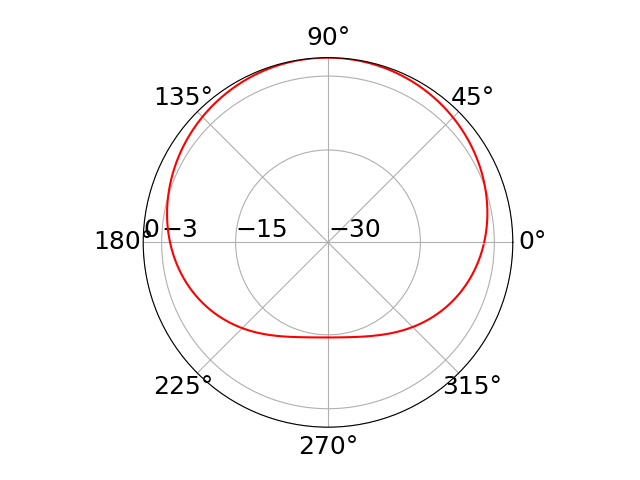
\includegraphics[width=0.49\textwidth]{figures/3DHorn_CAD_0_5GHz_H_plane.png}
	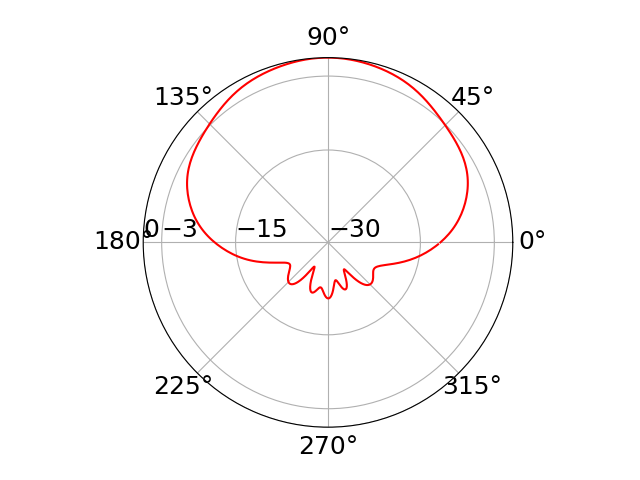
\includegraphics[width=0.49\textwidth]{figures/3DHorn_CAD_5GHz_H_plane.png}
    \caption{Radiation pattern results using open CAD for (top left) E-plane at 0.5 GHz, (top right) E-plane at 5.0 GHz, (bottom left) H-plane at 0.5 GHz, (bottom right) H-plane at 5.0 GHz.}
\end{subfigure}
\hfill
\begin{subfigure}{0.3\textwidth}
    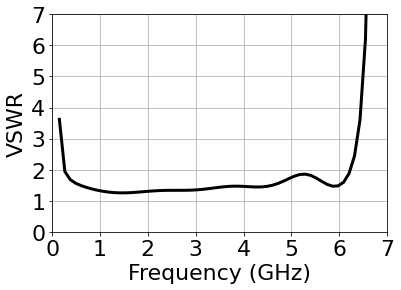
\includegraphics[width=0.99\textwidth]{figures/vswr.png}
	\caption{VSWR versus frequency in GHz for the RF horn.}
\end{subfigure}
\caption{Results for 3D RF horn design with MEEP and open CAD amenable to 3D printing.}
\label{fig:3d_cad}
\end{figure}

\subsection{RF Laboratory Capability and Prior ONR Funding}

We have established an Educational Partnership Agreement (EPA) between NSWC Corona and Whittier College.  One of the many advantages of the partnership is the technology transfer between NSWC Corona and Whittier College.  NSWC Corona has provided RF bench testing equipment that is perfectly suited to the proposed work.  More details are provided in our Facilities, Equipment, and Other Resources documentation.  Additionally, residual funds from our start-up grant have been used to purchase a System76 Thelio desktop system capable of performing our initial CEM calculations.  Our laboratory is therefore well-equipped to complete the proposed work, and this minimizes budgetary impact.  

This research has been completed with significant contributions from diverse undergraduates.  We summarize the personnel funding contributions to the early stages of this work in our Facilities, Equipment, and Other Resources documentation.  The researchers have diverse majors and interests, including our 3-2 Engineering, Physics, Mathematics, and Math/Integrated Computer Science programs.   After Whittier College, these students have begun roles with the Laser Interferometer Gravitational-Wave Observatory (LIGO) Collaboration, the University of Southern California (USC), and The Aerospace Corporation.  Whittier College has a strong track record of providing access to higher education, and careers in science and technology, to traditionally underrepresented students.  If our proposal is successful, these students will be exposed to new pathways in CEM, engineering, physics, and geoscience.

\section{The Connection to Ultra-High Energy Neutrino Observations}
\label{sec:askaryan}

The flux of neutrinos with energies between [0.01-1] PeV ($10^{15}$ eV) has been detected by IceCube \cite{10.1126/science.1242856}.  The UHE-$\nu$ flux, with energies above 1 PeV, could explain the unknown origin of UHE cosmic rays (UHECR) \cite{Ackermann:201946d}.  This flux also represents an opportunity to study electroweak interactions at record-breaking energies \cite{Ackermann:20195ec}.  Previous analyses have shown that the discovery of UHE-$\nu$ will require an expansion in detector volume, because the UHE-$\nu$ flux is expected to decrease with energy (see \cite{10.1103/physrevd.99.122001,10.1088/1475-7516/2020/03/053,10.1103/physrevd.98.062003} for current energy-dependent upper limits on UHE-$\nu$ flux).  Whereas the IceCube detector currently observes neutrinos via optical signals that travel $<100$ m, the Askaryan effect translates a UHE-$\nu$ interaction into an RF pulse that travels more than 1 km in dielectric media such as Antarctic and Greenlandic ice \cite{askaryan1,zhs,10.3189/2015jog14j214, 10.3189/2015jog15j057, 10.1016/j.astropartphys.2011.11.010}. 

Utilizing the Askaryan effect therefore allows for detectors with vastly larger effective volumes than optical observations.  Arrays of $\mathcal{O}(100)$ \textit{in situ} detectors encompassing effective areas of $\approx 10^4$ m$^2$ steradian per station, spaced by $\mathcal{O}(1)$ RF \textit{attenuation length} could discover a UHE-$\nu$ flux beyond the limits of the EHE analysis.  Polar ice formations in Antarctica and Greenland have the longest RF attenuation lengths.  A group of prototype Askaryan-class detectors has been deployed in polar regions that seek to probe unexplored UHE-$\nu$ flux parameter-space \cite{rice,10.1088/1475-7516/2020/03/053,10.1103/physrevd.102.043021,10.1103/physrevd.99.122001}. 

Askaryan radiation was first observed in laboratory settings \cite{saltzberg,10.1103/PhysRevD.74.043002,ask_ice}.  Working with an undergraduate researcher, we recently published a theoretical model of the electromagnetic field of Askaryan radiation \cite{PhysRevD.105.123019}. Askaryan models are incorporated into simulations like AraSim in order to calculate expected signals and aid in detector design \cite{dookayka2011characterizing,testbed,10.1140/epjc/s10052-020-7612-8}.  Software developed for IceCube Gen2 (radio) utilizes machine learning and the Askaryan pulse shape to reconstruct UHE-$\nu$ properties in future data \cite{10.1140/epjc/s10052-019-6971-5,10.1088/1748-0221/15/09/p09039,IFT}.  Askaryan electromagnetic fields are combined with RF channel responses to form ``signal templates'' used to search large data sets for signal candidates \cite{10.1088/1475-7516/2020/03/053,10.1016/j.astropartphys.2014.09.002}.  Data sets are large for Askaryan-class detectors due to RF thermal backgrounds, while  Askaryan signal SNRs at RF channels are expected to be small (SNR $\approx 3$) \cite{10.1088/1475-7516/2020/03/053,rno}.  Signal template matching is a powerful technique for noise rejection and signal identification \cite{10.1016/j.astropartphys.2015.04.002,10.1016/j.astropartphys.2014.09.002,barwick2016radio,10.1088/1475-7516/2020/03/053}. 

Given the expected signal SNR, phased arrays have been incorporated into Askaryan-class prototype detectors \cite{Vieregg_2016,AVVA201746} to increase the UHE-$\nu$ detection probability.  Examples of this strategy are ARA5 \cite{PhysRevD.105.122006}, and the first deployments of Radio Neutrino Observatory, Greenland (RNO-G) \cite{rno}.  The arrays in each consist of identical, vertically polarized dipoles.  These design choices were made for mechanical reasons, because the array must fit in a 100 m deep, vertically-drilled borehole in the ice.  The radiation pattern exhibits azimuthal symmetry, and there is \textit{minimal sensitivity to the horizontal Askaryan field component}.  Further, the designs assume a uniform index of refraction for the ice surrounding the array.  As part of our proposed work, we seek to use machine learning to discover horizontally polarized array designs that fit into the borehole and account for the index of refraction, $n$.  

We included a short study of phased array behavior in the South Pole ice environment in our recent publication \cite{electronics10040415}.  Most commercial CEM packages assume a uniform $n$ in the surrounding medium.  By contrast, MEEP gives the user 3D control of the index of refraction, $n(x,y,z)$.  In polar environments, $n$ varies with the depth ($z$) near the snow surface.  The $n(z)$ function is well-measured in Antarctica \cite{horizPaper}, and Greenland \cite{deaconu_2018}.  ARA (South Pole), RNO-G (Greenland), and IceCube Gen2 (radio) (South Pole) can all benefit from designs that account for $n(z)$ and have sensitivity to the \textit{horizontal} component of the Askaryan field. There is an ongoing effort to reconstruct the horizontal and vertical components of polarized test signals through South Pole ice, in order to more tightly constrain future UHE-$\nu$ observations \cite{10.1088/1748-0221/15/09/p09039}. 

The common simulation package used for ARA, RNO-G, and IceCube Gen2 is now NuRadioMC, built from prior experience with ARA and ARIANNA \cite{10.1140/epjc/s10052-020-7612-8,10.1109/tns.2015.2468182,10.1016/j.astropartphys.2011.11.010,Barwick:2014pca,10.1103/physrevd.102.043021}.  NuRadioMC addresses analytically the ray-tracing solution for UHE-$\nu$ signals as they propagate through polar ice.  We derived the analytic ray-tracing solutions presented in \cite{10.1140/epjc/s10052-020-7612-8} and \cite{horizPaper}, which were adopted into NuRadioMC.  A goal of our proposed research will be to incorporate realistic, 3D field propagation into NuRadioMC using FDTD computations with MEEP, with our analytic Askaryan model as the MEEP source \cite{PhysRevD.105.123019,10.22323/1.395.1217}.  This integration should boost the accuracy of the computations made with NuRadioMC, which will be matched with future ARA, RNO-G, and IceCube Gen2 data to isolate UHE-$\nu$ signals.

\section{The Connection to Remote Sensing of Ice Sheets}
\label{sec:cresis}

A gap exists in Askaryan-based UHE-$\nu$ science that connects to the remote sensing of ice sheets.  A knowledge of the RF attenuation length, $\lambda$, versus frequency, depth, and location is paramount to understanding UHE-$\nu$ detector sensitivity.  Although detailed measurements of $\lambda$ versus frequency have been made in Antarctica and Greenland \cite{aguilar_2022,10.3189/2015jog14j214,10.3189/2015jog15j057,barwick_besson_gorham_saltzberg_2005}, $\lambda$ has not been measured as a function of geographic location: $\lambda(x,y)$.  Further, $\lambda(z)$ is merely inferred from depth-averaged attenuation measurements and ice core temperature data (see Fig. 24 from \cite{10.1016/j.astropartphys.2011.11.010}). IceCube Gen2 (radio) will require $\lambda(x,y,z)$ to be measured.  CReSIS radio sounding data, available on the Open Polar Server (OPS), have been used to constrain $\lambda(x,y)$ across Greenland \cite{10.1002/2015rs005849}.  Far less CReSIS data is available near the South Pole, due to the complex logistics of organizing flights in that region.  Such logistical challenges are motivating a new effort to incorporate radio sounding instrumentation into unmanned aerial systems (UAS). 

UAS enrich radio sounding data for geophysics and partricle astrophysics.  In the past, radio sounding data has been generated from human-piloted fixed-wing aircraft carrying on-board radar.  Flight lines can be hundreds of kilometers long, scanning wide areas with synthetic aperature radar (SAR) techniques.  There are, however, three key disadvantages.  First, there may not be a flight near the desired location (e.g. South Pole).  Second, flights only give a snapshot, and may not return to the site for years.  Third, the radar bandwidth does not always overlap with the science bandwidth of (for example) IceCube Gen2.  Dedicated UAS could constrain $\lambda(x,y)$ in both the temporal and spatial regimes.  UAS are able to hover and fly at lower altitudes, so they can collect a wider variety of data than fixed-wing craft.  For example, the CReSIS ultra-wide band (UWB) Snow Mini radar system was integrated onto the AeroVironment Vapor 55 UAS.  The low altitude flight increases the SNR in difficult areas by pushing clutter angles outside the field of view.  The SNR is also boosted by hovering due to increased integration time over the site \cite{arnold_2020}. The average cost of the Vapor 55, however, is about \$$90$k USD.  

In our RF design lab at Whittier College, our group has already constructed a 3D printed drone using PLA filament and commerical parts.  The unit has $\approx 1$ kg payload and a 20-min flight time.  The total cost is $\approx 1$k USD (see Fig. \ref{fig:drone}).  Before the COVID-19 pandemic paused in-person work, we had plans to equip it with solar charging and cold-temperature components.  Thus, there is a potential for collaboration between CReSIS and IceCube Gen2 (radio) to solve a common problem: the solar rechargeable $\lambda(x,y)$ measurement system with vertical take-off and landing (VTOL).  Our drone design with VTOL capability can be 3D printed and assembled from commercial parts for \$$\approx1$k.  We will study how our colleagues in CReSIS outfit UAS models for cold temperatures.  We will undertake the task of incorporating solar charging, relying on our experience from ARIANNA and ARA.  When outfitted with a 3D-printed phased array radar, we will have a formidable system capable of filling gaps in our knowledge of polar ice sheets.  

\begin{figure}
\centering
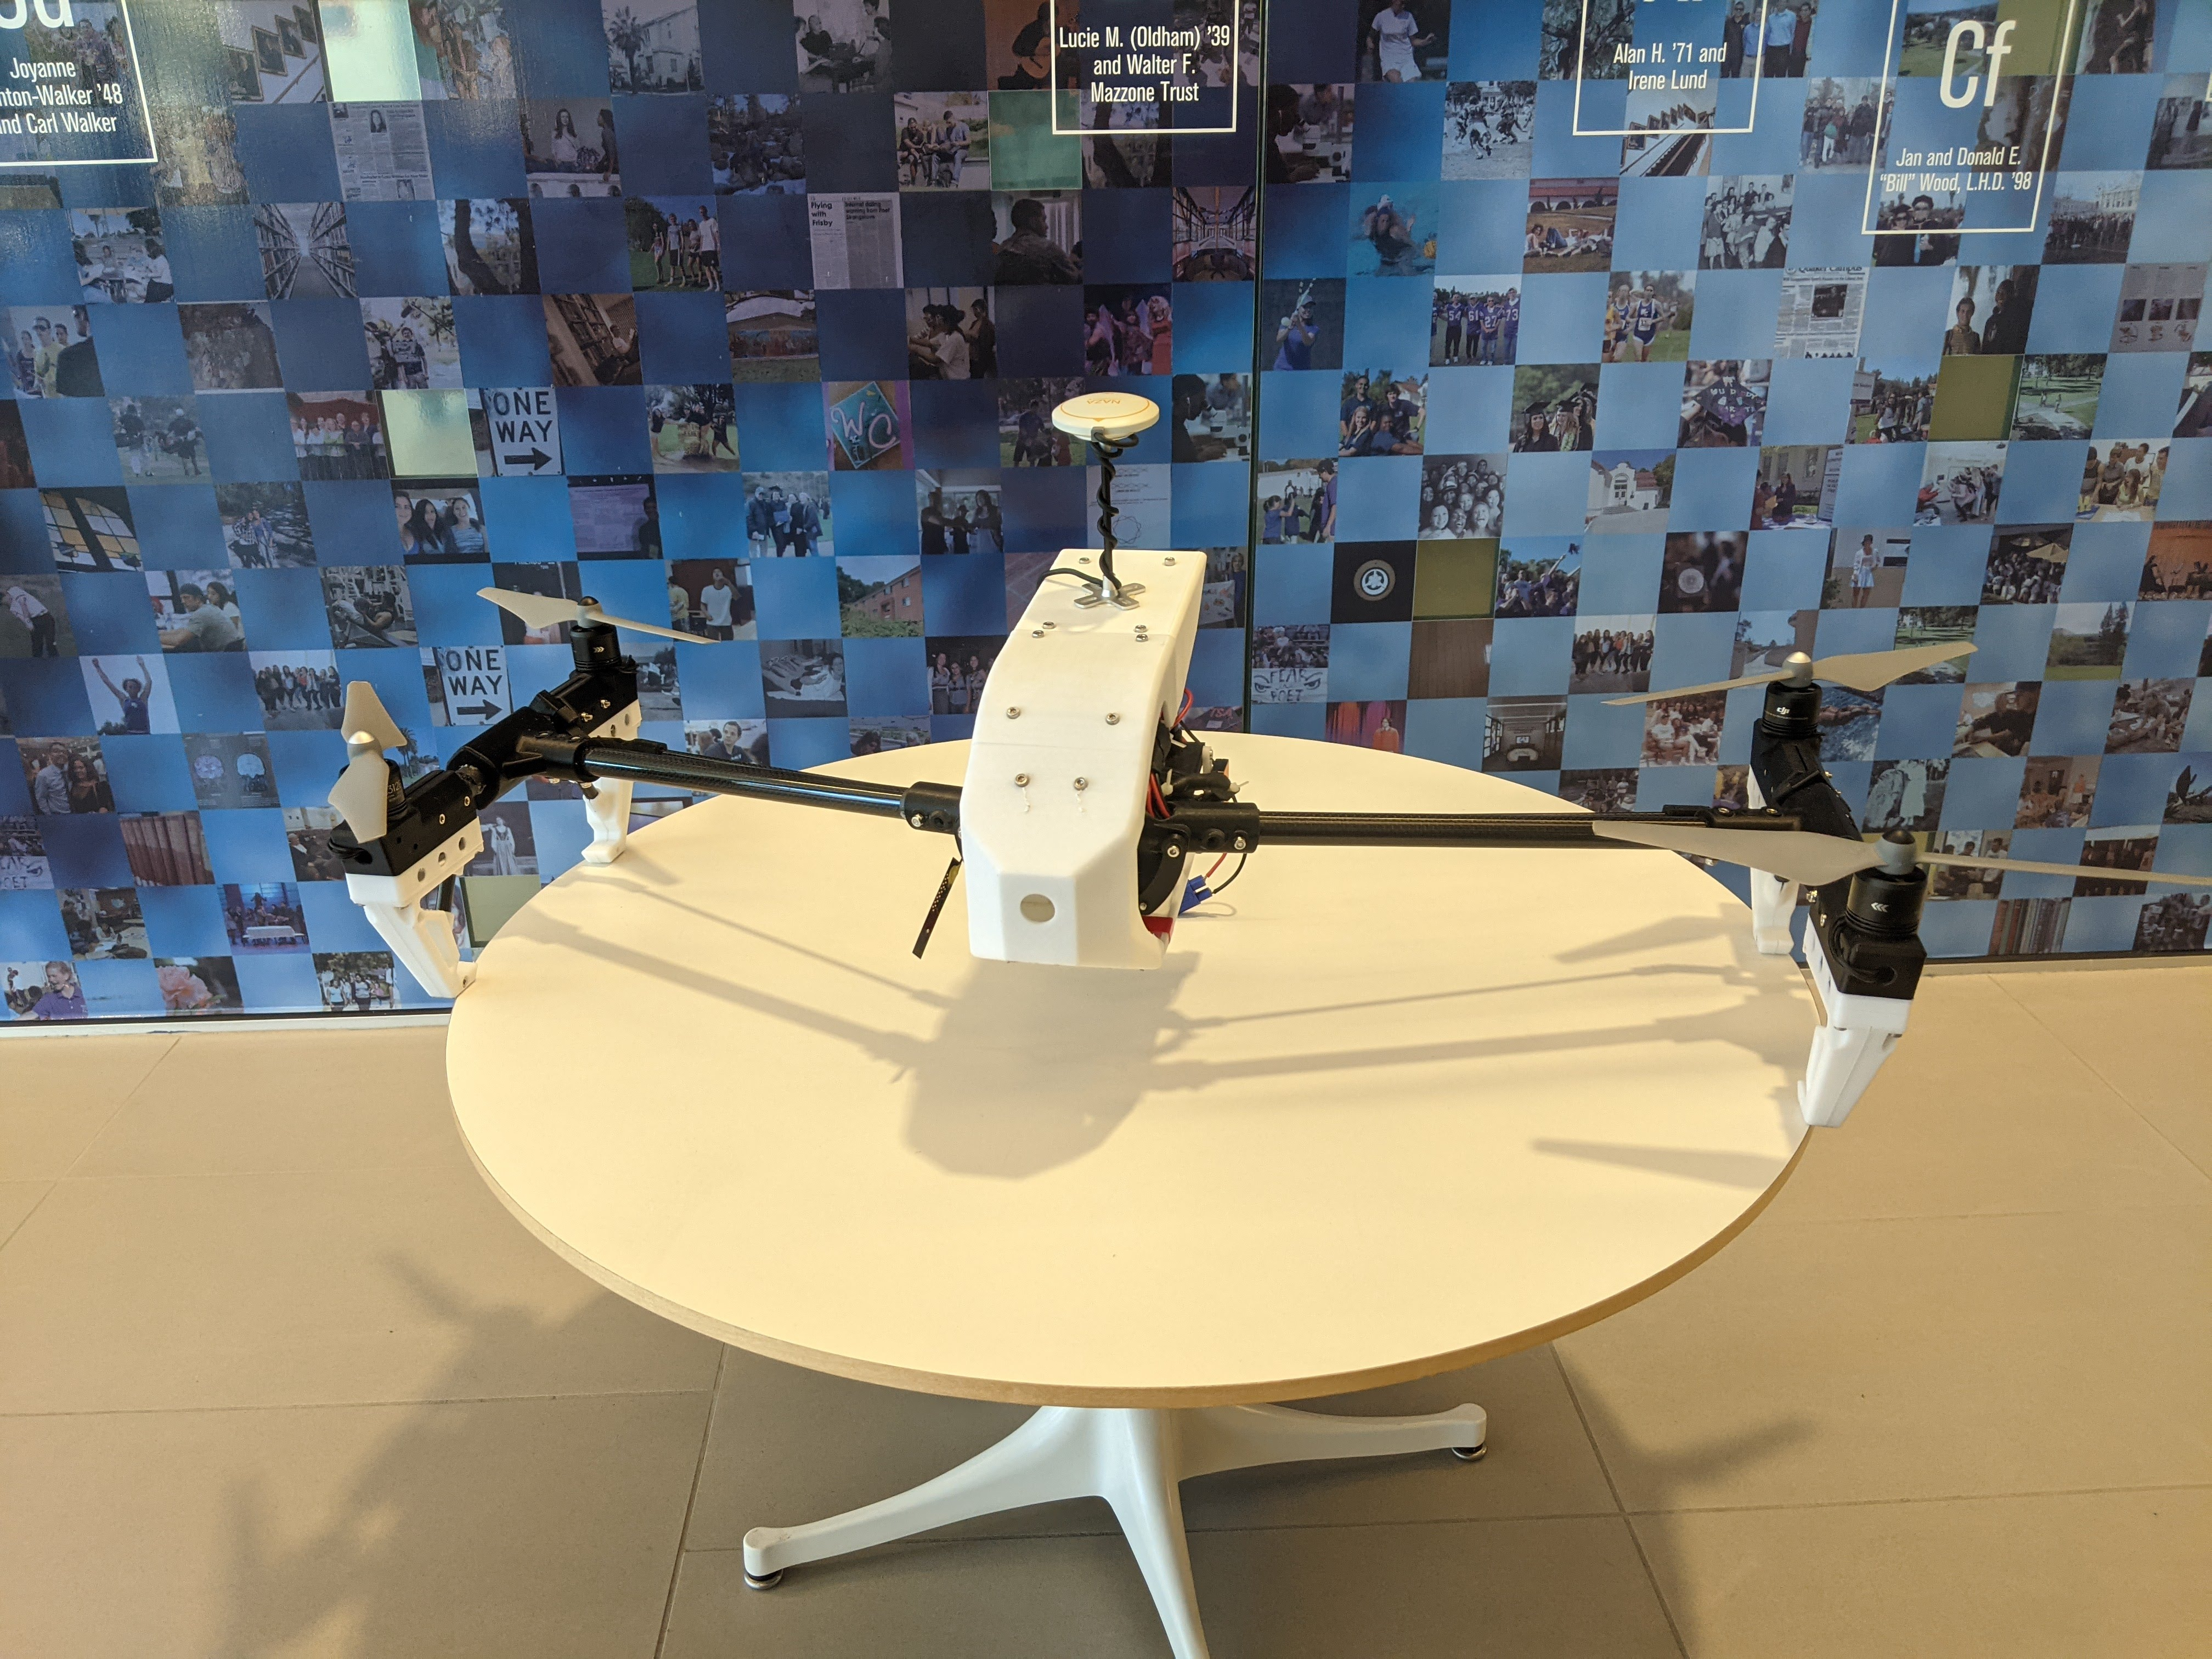
\includegraphics[width=0.4\textwidth]{drone.jpg}
\caption{\label{fig:drone} Our 3D-printed quad-rotor drone, designed and assembled by Whittier College undergraduates.  The drone is equipped with hand-held RC and laptop control, and GPS.}
\end{figure}

The incorporation of phased array radio sounding systems on UAS faces an optimization problem: the right balance between craft weight, thrust, payload, and flight time must be achieved.  To collect quality radio sounding data, the payload must be flown horizontally for $1-10$ km, implying $\approx 1$ hr battery life at reasonable speeds.  Longer flight times require larger batteries.  Increased battery size increases weight, which tends to decrease flight time.  Phased array payloads with a large number of elements could benefit data collection, but this adds weight and decreases flight time.  The optimization is made far easier if the phased array is integrated into the UAS hull.  We propose to study how the phased array can be printed into the UAS hull using machine learning to optimize beam-forming.  The Electrifi filament has a similar density to aluminum, meaning it can serve as \textit{both} a structural component and a phased array material.  Through this research, we seek to advance ongoing efforts to miniaturize radar for UAS radio sounding.  

As part of this engineering effort, we also propose to simulate expected results using MEEP.  Performing a CEM simulation that incorporates the ice properties and the UAS radar response would enrich the research in two ways.  First, such simulations enhance the design process, revealing design requirements, shortcomings, and ways to overcome them.  MEEP simulations require the user to specify the complex matrix for the dielectric constant of the medium, $\epsilon(x,y,z)$.  The $\epsilon$ matrix  determines how RF waves reflect, refract, and propagate back to the receiver.  Optimizing UAS phased array design for $\epsilon(x,y,z)$ measurement will result in optimal precision for $\lambda(x,y,z)$, because $\epsilon$ and $\lambda$ are related analytically \cite{10.3189/2015jog14j214}.  Second, building such MEEP simulations will provide a cross-check between the observed $\epsilon(x,y,z)$ from field data, and the simulated $\epsilon(x,y,z)$. 

FDTD simulations of sufficient precision for $\epsilon(x,y,z)$ and $\vec{E}(x,y,z,t)$ are notorious for consuming computational resources like volatile memory.  We have acquired a System76 Thelio desktop system with AMD Ryzen Threadripper 3990x 64-core, 128 thread processor.  The system has 0.5 GB of volatile memory per thread.  We have already shown that running MEEP in parallel on our system reduces run times by an order of magnitude \cite{meepcon2022}.  The reduction is due primarily to increased set up speed for $\epsilon(x,y,z)$.  Thus, we are in a position to perform these calculations quickly and efficiently.  Learning how to introduce parallelism into computational problems will also be of educational benefit to our STEM undergraduates at Whittier College.  In fact, the introduction of new concepts related to our research within STEM courses at Whittier College is a main goal of our proposal.

\section{Integration of Research and Education at Whittier College}
\label{sec:int}

The integration of our proposed reasearch into our STEM curriculum will benefit our diverse undergraduates in two ways.  The first benefit is the enrichment derived from integrating applications of our research into our courses.  The second benefit is the creation of undergraduate research opportunities, providing a venue for students to grow and apply their skills.  Our goal is to perform course integrations within the Departments of Physics and Astronomy, and Mathematics and Computer Science.  We have faculty in these departments who specialize in machine learning, and who are therefore well-positioned to incorporate this material.  For example, Prof. Fred Park specializes in the application of machine learning and parallel computing to computer vision and image analysis \cite{SHI201528,doi:10.1137/20M1337041}.  Whittier students regularly perform reearch with faculty, and we have fellowship programs to support them.  Our students have made wonderful achievements in CEM, firmware design, and theoretical physics with our local Ondrasik-Groce and Fletcher Jones Fellowships.  Our goal is to expand this practice through NSF-sponsored opportunities, funded through our proposed work.

\subsection{Course Integrations - Electromagnetism and Computational Physics}
\label{sec:integration}

Course integrations that will take place within the Department of Physics and Astronomy are Algebra-Based Physics II (Electricity, Magnetism, and Modern Physics), Calculus-based Physics II (Electromagnetism), Electromagnetic Theory, Optics, and Computational Physics\footnote{I personally teach Algebra-Based Physics II, Calculus-Based Physics II, and Electromagnetic Theory.  Optics and Computational Physics are normally taught by my colleagues within Physics and Astronomy.  Computational Physics will soon be handed to myself and others as the usual instructor retires.}.  The first two courses represent introductory level content on electromagnetism.  Web-based learning modules will be developed to illustrate electromagnetic waves and optics via MEEP in Jupyter notebooks.  Jupyter is a cross-platform open-source project that supports interactive data science and scientific computing.  We have experience creating and sharing MEEP notebooks in Jupyter to accomplish research \cite{electronics10040415}, and in teaching Computer Logic and Digital Circuit Design using the PYNQ-Z1 SoC. The primary learning enhancement is to illustrate dynamic electromagnetic fields, shown alongside textbook examples.  The students can therefore compare their theoretical understanding with a visual representation.  Their final projects are self-designed experiments in DC circuits, optics, and magnetism.  We look forward to students accepting the challenge of matching simulation output to their real-world results. 

We submit analyses of our teaching every two years as part of our tenure and promotion process.  These analyses have revealed the value of the synergies between traditional lecture content, simulations, and lab experiments.  Students in introductory courses are prepared to apply concepts in their own projects when the ideas solidify in their minds.  Solidification occurs when they demonstrate them as theoretical predictions, simulate them, and test them in the lab.  After solidification, learning anxiety fades, and students feel comfortable applying concepts.  A good example is DC circuit analysis.  We solve systems of equations that predict currents through multiple devices connected to a battery.  We use the PhET DC Circuit Construction Kit to simulate current in the circuit, and students can measure current in the simulation.  The students replicate the virtual circuit in the lab, and show that the results match the simulation.  There are, however, few HTML5 PhET simulations that illustrate dynamic electromagnetic fields.  We will use Jupyter modules with MEEP to fill this gap, completing the synergy for electrodynamics. 

There are three advanced physics course amenable to integration: Optics, Electromagnetic Theory, and Computational Physics.  Our Optics course introduces students to three areas.  The first is ray optics, with discussions of lenses and optical instruments.  The second is wave optics, with discussions of superposition, interferance, and diffraction. The third is modern optics, with discussions of photons, spectra, lasers, interferometry, fiber optics, and nonlinear optics.  One useful Jupyter module incorporating MEEP into ray and wave optics would be a lens example demonstrating focal length.  As the course progresses to modern optics, the lens example could be augmented to illustrate examples from photonics and machine learning \cite{meepcon2022_3}.  Some examples include flux and spectral monitoring for diffraction gratings \cite{meepcon2022_4}, and waveguides for fiber optics \cite{meepcon2022_5}.  Most Optics students have taken Computer Science 1 (Python3) and Modern Physics, so combining Python and electromagnetism should be achievable.  To integrate CEM into Optics, I will collaborate with the instructor, Prof. Serkan Zorba.  

The course integration in Electromagnetic Theory carries great potential.  This one-semester course covers chapters 1-7 of \textit{Introduction to Electrodynamics} by D. Griffiths (Cambridge University Press, 2017), with some examples of electromagnetic waves.  Students are first exposed to electromagnetic waves in a vacuum in the prerequisite Modern Physics.  Using Jupyter modules, we can introduce waves interacting with non-uniform dielectric media.  The difference between ray-tracing and true 3D propagation in polar ice with $n(x,y,z)$ is an excellent example of how the UHE-$\nu$ research, CEM, and teaching intersect (see Sec. \ref{sec:askaryan}).  Many examples in the rich MEEP documentation can be adapted for these modules.  One example, ``the S-parameters of a directional coupler,'' is a system of waveguides that provided basic code for computing the S-parameters of our RF antenna CAD designs \cite{meepcon2022}.  Finally, we can introduce a Jupyter module illustrating diffuse reflection from rough surfaces.  This module will form a connection between CReSIS radio sounding research, CEM, and teaching (see Sec. \ref{sec:cresis}).  

\subsection{Course Integrations - Computer Logic and Digital Circuit Design, and Digital Signal Processing}

I have created two computer science courses at Whittier College: Computer Logic and Digital Circuit Design, and Digital Signal Processing.  The former covers number systems, Boolean algebra and complex logic functions, adders/encoders/comparators, shift-registers/memory/counters, finite state machines, ADC/DAC, firmware programming with Python, and lab techniques with digital circuits.  Laboratory activities are performed on the PYNQ-Z1 SoC, allowing students to write firmware in Python.  Examples include creating digital logic functions with LED outputs, and ADC/DAC behavior with Digilent PMODs.  There are a plethora of examples with the PYNQ community that implement neural networks and image/video processing using FPGA acceleration.  We know the students seek experience in machine learning applications.  A useful course integration is to mix FPGA acceleration, machine learning, and CEM calculations into a learning module that can be expanded into a student-designed final project.  It is indeed possible to run Jupyter, MEEP, and FPGA acceleration code simultaneously on the PYNQ-Z1 SoCs.  Adding this module will enhance education \textit{and} research, because the students will discover how to accelerate CEM with FPGAs.

Digital Signal Processing (DSP) covers many topics that naturally follow Computer Logic and Digital Circuit Design.  We cover statistics, probability, complex numbers, noise, ADC/DAC, and sampling and digitization.  We also cover Fourier series and transforms, discrete Fourier Transforms (DFTs), Laplace and z-transforms, linear time-invariant (LTI) systems and filtering, and audio/image processing.  DSP and Computer Logic and Digital Circuit Design take the students all the way from basic binary to understanding digitized, sampled signals with complex analysis.  An interesting course integration between DSP and our CEM research is the application of DFTs to MEEP flux monitors and near-to-far-field monitors.  These are objects that compute and project the radiation flux passing through a surface as a function of frequency using DFTs.  Students will learn that the radiation is simply a sampled signal within a CEM context, and that the DFT is a tool for understanding spectra.  We can adapt Jupyter modules we have already written to this task. 

\subsection{Course Integrations - Introduction to Data Science with Python, and Machine Learning}

Introduction to Data Science with Python, and Machine Learning represent the final two course integration opportunities.  The former is an introductory course in which students learn import, explore, analyze, and visualize data using tools like Jupyter notebooks, NumPy, and Matplotlib.  More advanced tools like Pandas, SciPy, and scikit-learn are also introduced.  There are several straightforward enhancements that can be provided with Jupyter notebooks that demonstrate CEM.  Quantities like radiation patterns and S-parameters are fertile grounds for learning to visualize data with Matplotlib.  We have published such visualizations, and we can share this experience \cite{electronics10040415}.  Scikit-learn is already included in the syllabus, so RF antenna optimization with basic machine learning tools is also straightforward.  This course is taught by Prof. Glenn Piner, in the Department of Physics and Astronomy.  By working together to incorporate our proposed work into Introduction to Data Science with Python, students will gain early preparation to contribute to future research.  

The final course opportunity for course integration is Machine Learning.  Typically taught by Prof. Fred Park, this course assumes a more advanced knowledge of Python and Calculus II.  Topics include unsupervised and supervised learning, data clustering, principle component analysis, logistic regression, support vector machines, neural networks, and deep learning.  One topic that might prove a useful addition to the syllabus is \textit{genetic programming}.  Genetic programming has been used to optimize RF antennas \cite{2016MsT.........58S,genetic}.  We will work together to incorporate genetic programming and other techniques into the syllabus.  We seek to demonstrate practical applications of machine learning in the fields of physics, geophysics, and climate science.  This course is in high demand because students understand the opportunities that await them in the defense and software sectors in Southern Californa.  One such opportunity will be our newly established EPA with NSWC Corona.  Our students will be doubly prepared with the engineering experience from the RF application, and the machine learning training.

\vskip 1.0\linespacing
\centerline{\bf \Large Project Description: Broader Impacts}
\vskip 1.0\linespacing

\section{Translation of STEM Research for our Community}
\label{sec:broad}

In the long run, our proposal will provide valuable opportunities to diverse students from our community, which is heavily influenced by our bilingual families.  Families that speak Spanish at home and English at school are very common at Whittier College (an HSI).  For Fall 2022 admitted students, 36\% are Hispanic/Latino, and another 8\% are International students.  According to our internal research, students of color and first-generation students represent 63\% and 29\% of the student body, respectively.  We have observe that students of color receive lower grades than their peers in our STEM courses (see Tab. \ref{tab:grades}).  We have learned from workshops that emphasizing the dignity and self-efficacy of the student works againts disparity \cite{cottrell1,cottrell2}.  In keeping with the project theme of \textit{translation} of progress in one area to serve another, and in order to emphasize the dignity of our students no matter their background or the adversity they encounter, we seek to produce a bilingual mobile application introducing STEM concepts within a welcoming digital environment. 

\begin{table}
\centering
\begin{tabular}{c c c c}
Discipline & GPA (Students of Color) & GPA (White) & Shift \\ \hline
Physics & 2.62 & 3.15 & -0.53 \\
Mathematics & 2.54 & 2.75 & -0.21 \\
Computer Science & 2.77 & 3.31 & -0.54 \\
Chemistry & 3.02 & 3.20 & -0.18 \\
Biology & 3.03 & 3.18 & -0.15 \\
Environmental Science & 3.17 & 3.25 & -0.08 \\
\end{tabular}
\caption{\label{tab:grades} GPA data for Whittier College students from Fall 2016 to Spring 2021, disaggregated by racial background and discipline.}
\vspace{-0.5cm}
\end{table}

Implementation of the Duolingo method for language and mathematics on a mass scale has provided promising results \cite{duolingo_whitepaper}.  Results presented within the educational data mining (EDM) literature provide additional examples of apps and techniques that boost engagement and success in introductory STEM courses \cite{edm1,edm2,edm3,edm4}.  Some members of our community have shared that translating mathematics and physics exercises into Spanish aids in solving them.  Our app will boost their skills and build confidence by offering them engaging, game-like physics training in the language of their choice.  Even if the base language of STEM content in our courses does not represent a barrier for our students, the design of our app, based on the Duolingo Method, should boost the skill of all our students. 

The Duolingo method has five components \cite{duolingo_whitepaper}.  The first is Learning by Doing, or utilizing the innate learning toolkit every student has.  Learning by doing also involves affordance-based design, embodied cognition, and explicit instruction.  The second component is to Learn in a Personalized Way.  This involves utilizing machine learning to ensure content is just difficult enough for the individual student to grow, but not so difficult that the student becomes disengaged.  The distinction hinges on ``desirable'' difficulty, versus ``undesirable'' difficulty.  The third component is to Focus on What Matters.  This component is about ensuring course content is matched to verified learning standards like Common Core.  The fourth component is to Stay Motivated.  Using game-like design with points, rewards, leaderboards, and collaboration has been shown to motivate students in a positive way.  The fifth is to Feel the Delight. This component is many things: quality storytelling, including diverse characters within the app, and providing moral encouragement.  The key is to create a positive environment conducive to learning.  

Two additional themes are relevant for mathematics learning in the Duolingo method: using multiple mathematical representations for the same concept (see Sec. \ref{sec:integration}), and the manipulation of tools.  Both themes follow the concrete-real-abstract (CRA) learning progression.  A CRA progression is used to guide students towards understanding abstract mathematical concepts by first introducing them with concrete tools or representations, and gradually increasing the level of abstraction.  According to the authors, ``Equations, pictures, and narratives can all be used to describe mathematical concepts.  Moreover, using multiple representations supports learners' analogical thinking abilities ... Because these representations also are at varying levels of abstraction, we construct lessons so learners experience representations which are closer to real objects before they interact with more abstract representations'' \cite{duolingo_whitepaper}. 

Once implemented, we have two goals for the app.  First, we seek to test the hypothesis that a bilingual Duolingo approach will boost the GPA results in Tab. \ref{tab:grades} and reduce disparities.  Second, we seek to affirm our students' dignity and cultural identity through the bilingual app design.  We will begin with English and Spanish, because these are the most common languages on campus.  I come from a bilingual family, and I can attest to the generational knowledge gap that would form if I tried to teach science to my family in English only.  We hope these twin goals will serve to build confidence in our students by welcoming them into STEM learning at the college level.  Finally, our app will be designed and built by Whittier College students for their peers.  We make this choice after participating in discussions with our colleagues on the Inclusion and Diversity Committee (IDC), and from attending seminars in Inclusivity in Introductory STEM Courses \cite{cottrell1,cottrell2}.  People naturally embed their identity and perspective in the systems and content they create.  They students themselves are the best source of ideas for structuring an app that bolsters the five tenets of the Duolingo Method.  

\subsection{Educational Application for Student Learning of STEM (EASTLOS)}

A prototype application, code-named EASTLOS for ``East Los Angeles'' (our geo-cultural area) is being built by Whittier College undergraduates.  The software and digital design of the app represents an opportunity for Whittier College students to enhance the learning experience for their peers while gaining valuable work experience.  We include paid student positions for code and digital design in our budget and project planning, and allocate time and space to finish the app.  By recruiting home-grown talent, we hope to inspire a passionate set of diverse software designers to help implement the app.  We include three general phases in our project planning (Sec. \ref{sec:time_im}).  First, we will design and implement the app for an introductory physics course.  Second, we will use the app to gather data and make improvements.  Third, we will present results to a broader audience, and help to implement the app in other courses and in the broader community. 

The first general phase is the design and implementation of a version that applies to an introductory physics course.  We will carefully recruit and interview coders and designers from the Whittier College community.  The pool of recruits consists of students majoring in Integrated Computer Science (ICS), Physics and Astronomy, Mathematics, Digital Art and Design, and members of the Whittier Scholars Program (WSP).  WSP is a program in which students design their own major, overseen by professors who guide the educational designs.  I serve on the WSP advisory board, and I have advised several WSP students to graduation.  I met one of my WSP majors in my Computer Logic and Digital Circuit Design course.  This student remixed our ICS and Physics majors into a program that ultimately produced a working bluetooth positioning system that ran on Android devices.  WSP students can have diverse skill sets that include both digital art and design, and software development.  Given my experiences, I forsee being able to recruit students from WSP, ICS and Physics who will make the app appealing and effective. 

The app will be bilingual in English and Spanish.  Our project planning calls for this translation to be done by a two-person team: a fluent undergraduate major in Spanish, and myself.  We will write the app in a local, student-friendly dialect, while keeping the language technically sound.  Sometimes technical ideas are expressed in different ways in two languages.  Good examples are physics word problems involving rates of change.  In English, one might say ``80 km per hour, for 4 hours.''  In Spanish, one might say ``80 kil\'{o}metros por hora, durante cuatro horas.''  Translated literally, this sounds like 80 kilometers for one hour, during four hours.  As the complexity of the word problem increases, we hypothesize that bilingual students can feel confusion.  The confusion stems from shifting between the interpretation of prepositions in two languages \textit{while} learning a new technical subject.  We would like to test the hypothesis that there are students in our community who measurably benefit when they can switch the exercise to their first language\footnote{Note that the widely-used OpenStax University Physics vols. 1-3, are now available in Spanish.}.

The second general phase of development will be to implement the app in an introductory physics course to collect student response and usage data.  Conservatively, we expect this to happen in the Fall semester of year 3 of the proposed project.  This gives us plenty of time to ensure smooth app functionality, integration of visual content, and to experiment with machine learning adaptation.  The app will be tested by students in algebra-based and calculus-based physics.  We will collect student usage data such as time spent per problem, total time spent on the app, accuracy for each exercise or activity, and number of attempts required to master an exercise.  The challenge is to fine-tune the underlying structure of the app to achieve the ``desirable difficulty'' discussed in the research cited in \cite{duolingo_whitepaper} (Learn in a Personalized Way).  

As part of this first run, we will invite feedback from the users.  Students can best share which features are helpful and which need to be improved or discarded.  We are especially interested in how the visual environment affects student performance.  After the prototype app is running successfully, we will focus on refining the visual design to account for student feedback.  For example, the Duolingo app uses diverse avatars that help teach language through stories and interactions.  We would like the students to \textit{see themselves} in the characters, thereby affirming their dignity and causing them to feel they belong in the course.  Thus, the work will take on a much more liberal-arts themed tone after this second phase.  At this point in the project, we will recruit digital art and design students to help achieve an aesthetic feel that is most natural and welcoming for our students.  Though this is outside the realm of physics and engineering, the educational literature shows that it makes a difference. 

The third general phase is the presentation and implementation of the app in the wider community.  We will begin by thoroughly reviewing the results from within our department, identifying any obvious trends or problems.  Once we reach consensus about the overall efficacy and proper role of the app, we can begin to use it within other introductory physics courses.  We have the perfect venue for sharing app results with our colleagues from other departments.  The Wardman Library Collaboratory at Whittier College regularly hosts faculty workshops on topics that include open educational resources (OER).  I have presented at these workshops twice (on the use of OER in physics and computer science), and the app results would fall under this category.  We hope to convince our colleagues of the merits of the approach by being transparent about the funcionality of the app.  By the Spring semester of Year 3 of the proposed project, we hope to present the results of the app to our wider Whittier community.  One way to achieve this is to present the app to general audiences at Whittier Public Library and East Los Angeles Library.  As the user base grows, we plan to make the app open-source while protecting our students' data.

\subsection{Bilingual Lecture Series and Recruitment for Whittier College}

As a final contribution towards the theme of \textit{translation} within our proposal, we will create bilingual lecture series about IceCube Gen2, polar research, and our open-source CEM research.  There are several high-profile IceCube members who are bilingual in English and Spanish, and we have bilingual contacts from the UHE-$\nu$ research community.  Thus, there is a pool of speakers we can invite to speak at Whittier College.  Once the app is ready for new users, we will present it to the community in a bilingual fashion at these same events.  The goal is to allow our students to see themselves in the speakers we invite, and learn about physics and engineering research.  Our undergraduate researchers can also present their work alongside the undergraduate translator. 

We will begin these lectures at Whittier College, and present with a similar style as the standard colloquium.  Most students will appreciate the bilingual aspect, but it will not be strictly necessary for understanding the material.  The focus will be more on identifying with the speaker and learning about new STEM research.  As we proceed into the broader Los Angeles community, it will not be hard to locate communities that do need both languages to maximize mutual understanding.  We do not have to locate these venues on our own, for Whittier College hosts the Center for Engagement with Communities (CEC).  The CEC has a long history of building community partnerships within Whittier, CA and beyond.  I have served the CEC Artemis Program twice, which is a program designed to connect young women from local high schools to STEM research at Whittier College.  Through CEC, we can form connections with local high schools and community organizations to share our work.

\section{Project Planning, Intellectual Merits and Broader Impacts}
\label{sec:time_im}

Our proposed project has many components that we now present as a cohesive, structured plan.  We have constructed a detailed five-year plan that includes all the integrated research and educational projects described in previous sections.  We share a breakdown of the plan here (illustrated in Tab \ref{tab:plan}), and we provide a detailed example in Fig. \ref{fig:gantt_1}.  In the interest of conciseness, we elect not to show all project planning charts for years 1-5.  The examples in Tab. \ref{tab:plan} and Fig. \ref{fig:gantt_1} are meant to convey that our progress will be assessed against concrete, measurable goals.  The data in Fig. \ref{fig:gantt_1} corresponds to just part of Project Year (PY) 1. 

\begin{table}[ht]
\footnotesize
\centering
\begin{tabular}{c | c | c | c}
PY & Project & Weight Factor & Time \\ \hline
1 & Hardware Acquisition & 10\% & Jul. '24 \\
 & Recruitment & 5\% & Sept. '24 \\ 
 & Student Training & 5\% & Sept. '24 \\
 & Course Integrations & 10\% & July '24, Dec. '24, Jan.-Aug. '25 \\
 & CEM/ML, RF Antennas & 10\% & Sept. '24 - May '25 \\
 & AM, RF Antennas & 10\% & Sept. '24 - May '25 \\
 & App Development, Android SDK & 10\% & Sept. '24 - May '25 \\
 & CEM/ML, Phased Arrays, Summer '25 & 20\% & May-Aug. '25 \\
 & AM, RF Antennas, Summer '25 & 20\% & May-Aug. '25 \\
\hline
2 & Hardware Acquisition & 5\% & Jul. '25 \\ 
 & Recruitment & 5\% & Sept. '25 \\
 & CEM/ML, Phased Arrays & 15\% & Sept. '25 - Dec. '25 \\
 & AM, Phased Arrays & 15\% & Sept. '25 - May '26 \\
 & App Development, Spanish translation and ML & 20\% & Sept. '25 - May '26 \\
 & \textbf{Publication in \textit{Electronics}} & 20\% & Jan. - Aug. '26 \\
 & CEM/AM for UHE-$\nu$, Summer '26 & 20\% & May - Aug. '26 \\
\hline
3 & Hardware Acquisition & 5\% & Jul. '26 \\
 & Recruitment & 5\% & Sept. '26 \\
 & CEM/ML, Drones & 15\% & Sept. '26 - May '27 \\
 & AM, Drones & 15\% & Sept. '26 - May '27 \\
 & Application Development, Data Collection & 20\% & Sept. '26 - May '27 \\
 & Application Development, Analysis, Summer & 20\% & May '27 - Aug. '27 \\
 & AM, Drones, Summer & 20\% & May '27 - Aug. '27 \\
\hline
4 & Hardware Acquisition & 5\% & Jul. '27 \\
 & \textbf{Publication in \textit{American Journal of Physics}} & 15\% & Jul. - Dec. '27 \\
 & Assessment of Course Integrations & 20\% & Jul. - Aug. '27 \\
 & AM, Drones & 20\% & Sept. '27 - May '28 \\
 & CEM/Simulation for UHE-$\nu$ & 20\% & Sept. '27 - May '28 \\
 & CEM/Simulation for UHE-$\nu$, Summer '28 & 20\% & May '28 - Aug. '28 \\
\hline
5 & Backlog Assessment & 10\% & Jul. '28 \\
 & CEM/Simulation for UHE-$\nu$ & 15\% & Aug. '28 - May '29 \\
 & Application Development & 15\% & Sept. '28 - May '29 \\
 & Backlog Fulfillment & 60\% & Aug. '28 - May '29 \\ 
\hline
\end{tabular}
\caption{\label{tab:plan} Project planning, for Project Years (PY) 1-5.  For detailed examples, see text and Fig. \ref{fig:gantt_1}. CEM: computational electromagnetism, ML: machine learning, AM: additive manufacturing.}
\end{table}

Table \ref{tab:plan} is a list of project tasks for PY 1-5.  Figure \ref{fig:gantt_1} contains calculations from our Gantt chart for PY 1 that correspond to project tasks, as an example of the analysis we have performed.  We have performed similar calculations for every project task in PY 1-5.  We give each project task a \textit{weight}, and a time span.  For example, hardware acquisition in PY 1 has a weight of 10\% and takes place throughout July of 2024.  The weights serve two purposes.  First, weights are used to determine the relative importance of finishing tasks and assigning workers appropriately.  Second, the PY completion percentage for a given year is calculated from a weighted average using the weights.  The task completion percentage is the average of the itemized sub-task percentages, weighted by the times required to complete them.  In Fig. \ref{fig:gantt_1}, the ``current date'' is 15-Dec-2024.  Hardware acquisition is completed on schedule.  Each sub-task is marked 100\%, with 0 required work days remaining.  The ``days to deadline'' numbers are negative when the due date has passed.  The CEM research is 50\% complete, from the itemized percentage data.  Accounting for just these two tasks, the project year is 15\% complete, 10\% hardware acquisition plus $50\% \times 10\%$ from CEM research. 

\begin{figure}
\centering
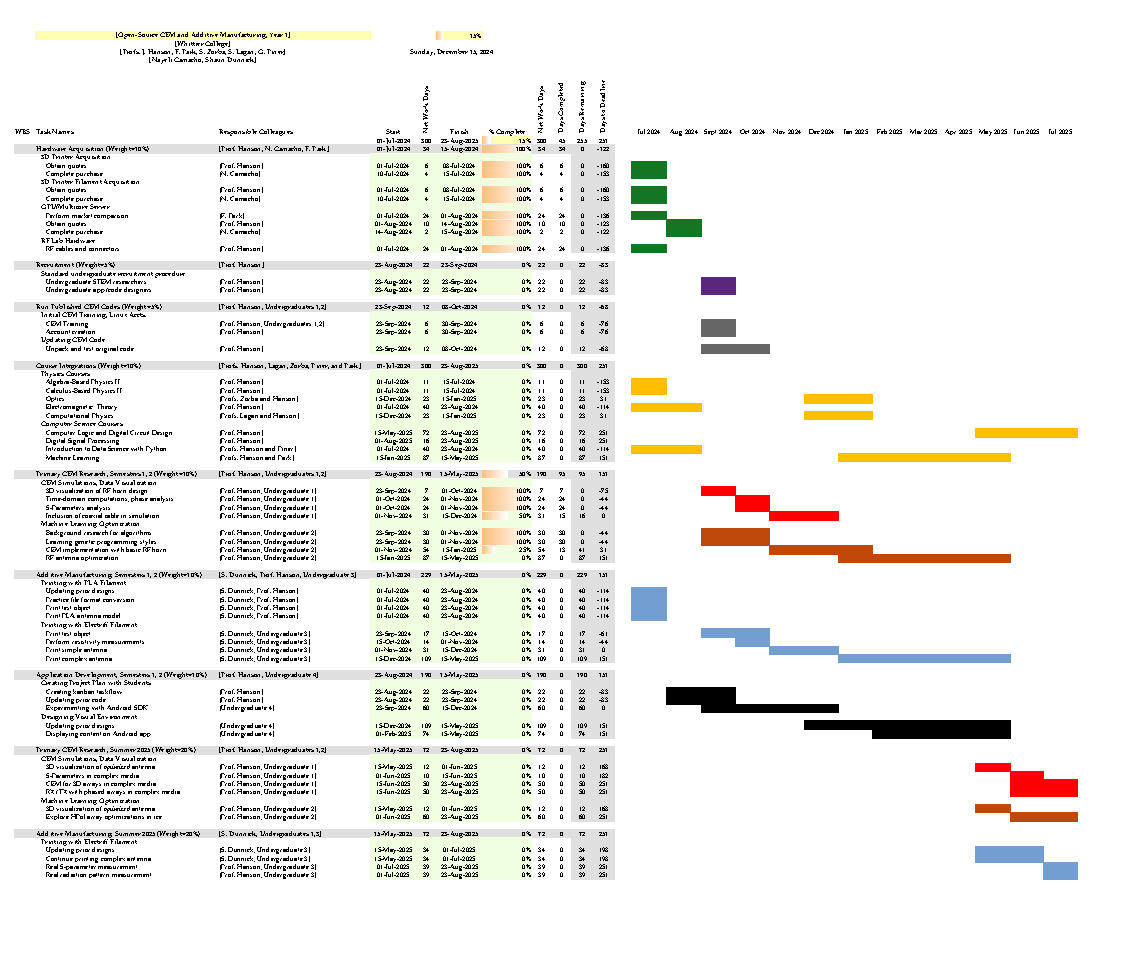
\includegraphics[width=0.99\textwidth,trim=0cm 12.2cm 8.5cm 1.25cm,clip=true]{project_planning/cem_project_gantt_yr1.pdf}
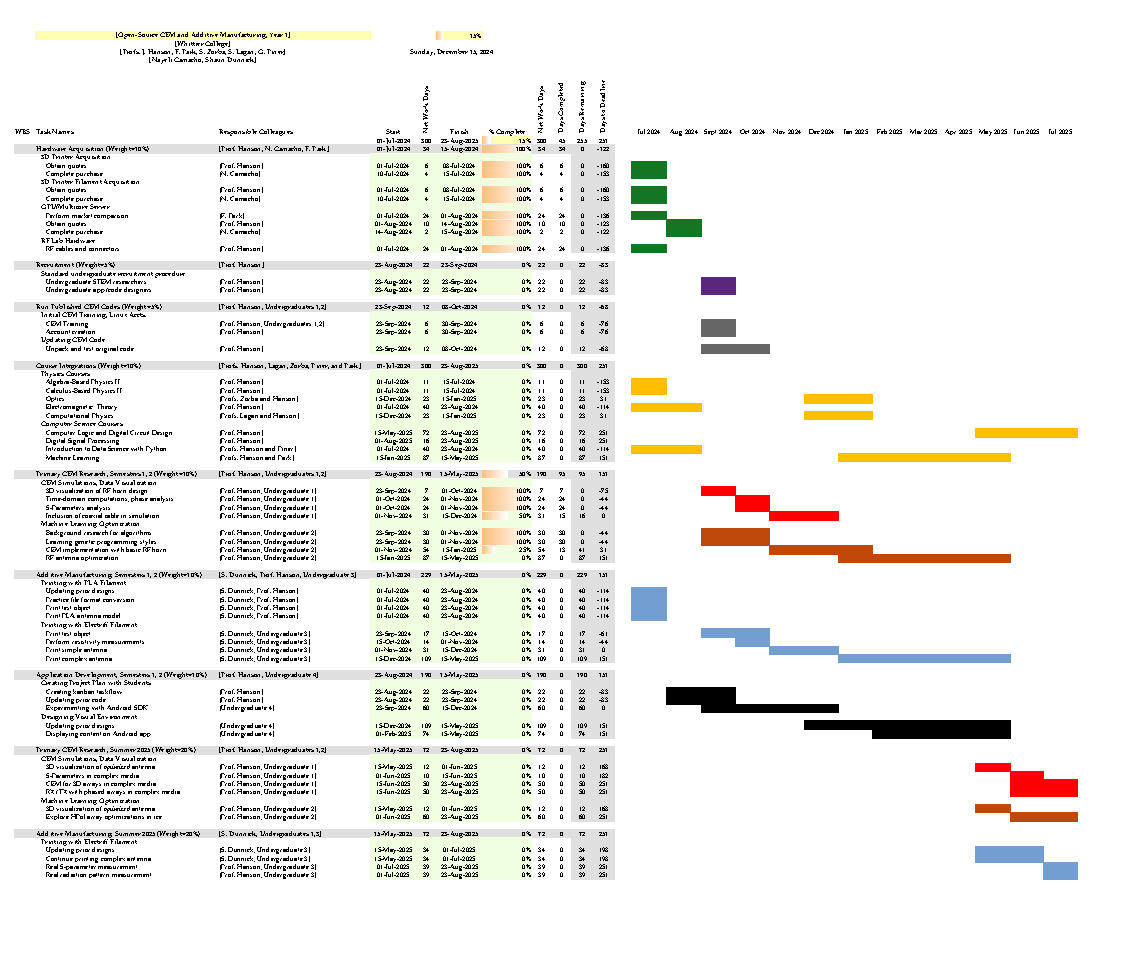
\includegraphics[width=0.99\textwidth,trim=0cm 7.0cm 8.5cm 7.9cm,clip=true]{project_planning/cem_project_gantt_yr1.pdf}
\caption{\label{fig:gantt_1} Aspects of Project Year 1 (academic year 2024-25).  See text for details.}
\end{figure}

We have made calculations similar to those in Fig. \ref{fig:gantt_1} for each project task in the general plan in Tab. \ref{tab:plan}.  Using the corresponding Gantt charts, we have performed three analysis checks.  First, we have ensured that the sum of my (Prof. Hanson) task weights in any given time period only rises above $50\%$ during Summer.  This is to ensure my time is not overloaded after accounting for my teaching load.  Second, we have verified that our plan is numerically self-consistent.  If each project task is completed, the correct weight is added to the PY completion percentage.  Numerical consistency prevents scheduling too much work with inadequate resources.  Third, we cross-checked the project plan with the proposal budget, to ensure we are recruiting the right number of undergraduate researchers for each Project Year.  This ensures we have adequate human resources to finish our work, while keeping the budget request under control.  Given these three checks, we believe our planning helps to maximize our productivity. 

Our plan includes six final products.  The first will be the 3D-printed RF phased array, geared towards UHE-$\nu$ science.  The second will be the course integrations to enhance our curriculum.  The third is the EASTLOS app for Android mobile.  The fourth product is a publication in the journal \textit{Electronics}.  The fifth product will be a drone design with integrated phased array designed with open-access CEM for geoscience.  The sixth product is a publication of EASTLOS data in the \textit{American Journal of Physics}.  In PY 5, we include \textit{backlog assessment} and \textit{fulfillment}.  During backlog assessment, we decide which incomplete projects gain priority.  Backlog fulfillment means finishing these projects.  Including backlog in our planning reflects the institutional wisdom of working with Whittier undergraduates, who sometimes have to prioritize course work.

After completing our project design for PY 1-5, we are fully aware that we may not achieve every project task.  Our plans call for undergraduate researchers to help complete project tasks.  They will be completing course work alongside our research and service work.  Knowing that undergraduates can be caught between course work and project tasks, we have decided to include two \textit{post-baccalaureate} positions in the project planning and budget.  These will be recent graduates with B.S. degrees in physics, computer science, or engineering that can help oversee and complete project tasks with myself and our undergraduate partners.  We do not assume we will complete every project task, but we have chosen a project plan that sets the bar high in order to achieve the maximum output for scientific progress and undergraduate education.

\clearpage

\section{Facilities, Equipment, and Other Resources.}

Whittier College is a HSI, with a mission to elevate undergraduate students from the communities of Los Angeles and beyond into academic achievement and scientific progress.  Piece by piece, we have established a research lab capable of supporting complex projects that merit NSF awards.  Part of this growth includes establishing a public-private partnership with a US Navy Lab called an educational partnership agreement (EPA).  Our EPA has facilitated technology transfers that will greatly benefit our proposed research.  Further, we have already used start-up grants to prepare for the work.  Finally, we have a strong tradition of privately funded undergraduate research fellowships at Whittier College, including the Keck Fellowship, the Fletcher-Jones Fellowship, and the Ondrasik-Groce Fellowship.  Having used these instruments to prepare our institution, we believe we are well-equipped to perform the proposed work.  We first describe the \textit{laboratory and office space} provided by Whittier College.  Second, we describe the \textit{computational resources} we have acquired that are relevant for the proposal.  Third, we discuss our \textit{additive manufacturing} resources.  Fourth, we discuss our \textit{RF testing and calibration} resources.  Finally, we focus on \textit{human resources} by demonstrating a track record of mentoring undergraduate researchers through research fellowships. 

\textbf{Laboratory and Office Space.} Whittier College has provided my group our own laboratory in our Science and Learning Center (SLC), completed in 2016.  This $30 \times 30$ ft. facility includes lab tables with power rails and ethernet, storage cabinets and drawers, a fume hood, a tool cabinet, and a closet.  This lab is home to our RF testing and calibration equipment, and it is a secure facility.  Several students can comfortably work alongside each other on electronics and engineering projects.  The lab has a variety of coaxial cables and electronics tools.  We have also been provided with a $40 \times 30$ ft. teaching laboratory.  During the academic year, the teaching lab is home to computer science and physics laboratory courses.  During the Summer, the lab is available for research, and is home to electronics tools and cables, and a soldering station.  Whittier College has also provided a $15 \times 15$ ft. machine shop.  The SLC machine shop is home to standard machine tools for traditional RF antenna construction, including a mill, lathe, drill press, band saw and safety equipment.  Finally, Whittier College has provided me with a secure office that is home to our System76 Thelio desktop computer. 

\textbf{Computational Resources.} Using our start-up grant, we acquired the System76 Thelio desktop system with AMD Ryzen Threadripper 3990x 64-core, 128 thread CPU.  The system has 0.5 GB of volatile memory per thread, 4.3 TB of permanent storage, and a NVIDIA GeForce GTX 1650 GPU.  The system was used in Summer 2022 to create our 3D open-source CAD models of broadband RF antennas, and to run the associated CEM computations in parallel.  Running our CEM calculations in parallel accelerated results by an order of magnitude.  Multiple on-campus users can utilize this system as a CEM server.  The number of simultaneous users or jobs is limited by the 0.5 GB of memory per thread.  The system can be easily upgraded to handle more users.  To facilitate scanning large parameter spaces for optimized phased array designs using machine learning, we will begin by using the Thelio system as a training ground for our more complex runs.  The Thelio can be easily upgraded with more memory and storage.  As the complexity of the research grows, we can expand to a more powerful system as neccessary.  Because of our experience with System76, we will perform market research on the System76 Jackal and Ibex GPU server lines before recommending upgrades.  

\textbf{3D Printing Resources.}  The SLC machine shop is also home to our MakerBot Replicator Z18, and we have since upgraded it with an Olsson Ruby extruder tip.  The ruby tip can withstand higher extruder temperatures without changing shape over time.  This makes it a better choice for 3D printing with the Electrifi filament we propose to use.  We are therefore equipped to start our project using the MakerBot 3D printer and the rolls of Electrifi filament already in our labs.  We plan to upgrade as necessary to Prusa and TriLab printers, since these are recommended by experts for use with the Electrifi metal-doped filament.  The SLC is home to staff in our department and the Department of Chemistry who have experience repairing and operating our 3D printer.  Thus, we are well-equipped to begin a multi-year project based on additive manufacturing with novel materials. 

\textbf{RF Testing and Calibration Resources.}  We have now begun an Educational Partnership Agreement (EPA) between Whittier College and a US Naval Research lab called NSWC Corona.  Through the technology transfer portion of the EPA, NSWC Corona has provided RF bench testing equipment that is perfectly suited to the proposed work.  A list of instruments transferred from NSWC Corona between 2020 and 2023 is shown in Tab. \ref{tab:fac}.  Our network analyzer and power sensors can perform S-parameter measurements over [9 kHz - 6 GHz] for our antennas under test (AUT).  Our signal generator can create calibration signals for our calibration antennas and AUT over [250 kHz - 6 GHz].  Our calibration antennas serve as benchmark devices for comparison to our 3D printed AUT.  Regular calibration is required for these devices, and our calibration kits serve this purpose.  Using our start-up grant, we have also acquired a Tektronix MDO 3024.  This mixed domain oscilloscope (MDO) is equipped with four analogue RF channels, and a fifth RF channel as spectrum analyzer.  The MDO 3024 can also accept 16 digital inputs simultaneous to the analogue channels.  The scope is perfect for low-frequency testing and verification of RF antennas and circuits.  Our laboratory is therefore well-equipped to complete the proposed work, and this minimizes budgetary impact.  The main area to upgrade is the bandwidth of the MDO 3024, which should be increased from 200 MHz to at least 1.5 GHz.  

\textbf{Human Resources.} Our research in CEM and additive manufacturing to date has been completed with significant contributions from diverse undergraduates.  We provide a summary of contributions from undergraduate personnel, and ONR faculty fellowships, to the early stages of this work in Tab. \ref{tab:fac}.  These researchers have diverse majors, including our 3-2 Engineering Program (Wildanger), Physics and Math double major (Hartig), and Math/Integrated Computer Science (G\'{o}mez-Reed and Householder), and Physics and Astronomy (Goodman and Smith).   These students have begun science and engineering roles with the Laser Interferometer Gravitational-Wave Observatory (LIGO) Collaboration, the University of Southern California (USC), and The Aerospace Corporation.  Whittier College has a good track record of mentoring undergraduate research fellows.  We seek to expand this practice through NSF-sponsored opportunities in additive manufacturing, CEM, and machine learning.  Finally, we have senior personnel who will help with the proposed work.  Lisa Newton is our Associate Director of Research and Sponsored Programs, and Nayeli Camacho is the administrator for Physics and Astronomy handling acquisition and purchase orders.  We also have Shaun Dunnick, a technician who helps maintain our 3D printing resources.  Our project planning analysis takes their valuable work into consideration.

\begin{figure}[hb]
\footnotesize
\centering
\begin{subfigure}{0.45\textwidth}
\centering
\begin{tabular}{c}
Equipment\\ \hline
Rohde and Schwartz ZVL6 Network Analyzer \\
Rohde and Schwartz NRP-91 Power Sensors (2) \\
Aeroflex 3416 Digital RF Signal Generator \\
Calibration antenna kits (2) \\
Calibration kits for Network Analyzer (2)
\end{tabular}
\end{subfigure}
\hspace{0.5cm}
\begin{subfigure}{0.45\textwidth}
\centering
\begin{tabular}{c c c}
Student/Professor & Grant Opportunity & Yr. \\ \hline
J. C. Hanson & ONR Faculty Fellow & '22 \\
D. Goodman & Summer researcher & '22 \\
A. Householder & Summer researcher & '22 \\
R. Hartig & Ondrasik-Groce Fellow & '22 \\
J. C. Hanson & ONR Faculty Fellow & '21 \\
A. Wildanger & Fletcher Jones Fellow & '21 \\
J. C. Hanson & ONR Faculty Fellow & '20 \\
R. Hartig & Fletcher Jones Fellow & '20 \\
J. P. G\'{o}mez-Reed & Ondrasik-Groce Fellow & '19 \\
J. P. G\'{o}mez-Reed & Keck Fellow & '18 \\
C. Smith & Keck Fellow & '18
\end{tabular}
\end{subfigure}
\caption{\label{tab:fac} (Left) RF testing and calibration equipment donated by NSWC Corona. (Right) Undergraduate researchers, and fellowships awarded to our group by year.}
\end{figure}

\section{Budget Justification}

We have crafted a budget that contains the personnel, equipment, and travel expenses required by the proposed project.  Our budget has been generated with the help of our Associate Director of Research and Sponsored Programs, and it reflects fringe benefits and other indirect costs associated with Whittier College.  With the professional help and advice of our colleagues, we have created a budget that provides for the project needs while aligning with appropriate budget guidelines.  Namely, the final figure does not exceed the minimum dollar amount specified for CAREER proposals within the Directorate for Engineering (ENG) by more than 10\%.  We first provide justification for our budget items in the personnel category.  Second, we describe our major equipment items.  Third, we describe our travel expenses.  We conclude with our remaining direct costs, comprised of smaller equipment purchases.  

\textbf{Personnel.}  The majority of our budget request is in the form of personnel salary and wages.  Due to the small size of our Department of Physics and Astronomy, we are not requesting academic year course releases.  Rather, our project plans call for undergraduate researchers to work with us throughout Project Years 1-5 to accomplish our work.  Thus, the only PI salary in our budget is 2 person-months per year for Summary salary.  Our project planning calls for undergraduate researchers during the academic year (AY), and summer research internships.  The average number of AY students we hope to recruit is 4 per year, but this number is modified depending on the Project Year.  For example, our Project Plan calls for an additional undergraduate worker in Project Year 2 to act as Spanish language translator for our EASTLOS application (see Project Description for details).  In Project Year 4, certain projects have already concluded.  Thus, our budget only calls for two AY researchers in Semesters 7 and 8.  Regarding the undergraduate Summer fellowships, we typically assume three per year, but in Project Year 2 we only require one student to finish the initial work accomplished in Semesters 1 and 2.  By performing this analysis, we intend to minimize budgetary impact while completing our work. 

In our personnel budget, we also include institutional wisdom gained after several years of mentoring undergraduates who have earned fellowships.  Whittier College is an undergraduate institution, meaning we lose the experienced juniors and seniors soon after we recruit them.  In other cases, first-year and sophomore recruits transfer to other institutions before a project finishes.  Thus, we have included ``post-baccalaureate'' researcher positions.  Paid at a higher rate, these recruits are meant to be recently graduated seniors looking to continue engineering work as their job search in the private sector progresses.  Other categories of students for these roles include students in our 3-2 engineering program, who leave Whittier College after three years, and students applying to graduate school. For students in these situations, we hope to retain talent for our project work, and to provide them with key experiences they will use in the workforce.  These students will be given some advisory and mentorship responsibilities as they work alongside their younger colleagues.  In this way, the budget reflects the organizational structure we will execute. 

\textbf{Major Equipment Items.} Our budget calls for two major pieces of scientific equipment.  The first is a Tektronix mixed-domain oscilloscope (MDO) with bandwidth greater than 1.5 GHz.  This will allow us to visualize received signals from antennas-under-test (AUTs) in the time-domain.  Collecting data in the time-domain, for example, will allow us to discover reflected signals that represent faulty coaxial cable connections between the AUTs and transmitters.  Though the MDO can provide frequency domain data, we already have a network analyzer capable of providing spectral information over a 6 GHz bandwidth.  We will use the network analyzer to collect S-parameter and radiation pattern data in the frequency domain.  Thus, the exploratory quotes we have obtained for the MDO focus on time-domain precision, number of RF channels, and measurement features in the time-domain.  The main driver of cost for MDOs is bandwidth, which must be $\geq 1.5$ GHz for our proposed designs. 

The next major equipment item reflects the need for computational resources.  There are two possible upgrades to our facilities that can achieve this goal.  First, we could purchase a new System76 GPU/multi-core server in either of the Jackal or Ibex product lines.  This new system would be used for machine learning and CEM calculations in service to our Project Plan, and for new computational research by our colleagues and students.  We envision a central server that will allow faculty from the Depts. of Physics and Astronomy, and Mathematics and Computer Science to perform computational work with job-scheduling.  Thus, we could utilize our System76 Thelio (see Facilities, Equipment, and Other Resources documentation) for initial CEM runs, and the shared server for calculations that require more power.  Prof. Fred Park (current chair of Computer Science and Mathematics Dept.) has the experience to utilize a GPU server for projects that would complement our research.  This approach bolsters our efforts to integrate our research and educational endeavors, for students could obtain server accounts used for course work in Machine Learning or Introduction to Data Science with Python. 

Alternatively, we could use the computational resources in the budget request to upgrade our System76 Thelio.  CEM calculations that use the FDTD approach are memory-intensive.  We could advance our CEM work with a memory upgrade to the Thelio, because this would enable more student accounts to run simultaneous jobs.  This approach would keep the computational work on our private desktop, meaning only students in our group would benefit.  However, this approach is simple and straightforward, requiring no server maintenance.  With either approach, the open-source CEM portion of our Project Plan will be accomplished.  Course integrations using heavy-duty computations could still take place, but in a more limited fashion for the courses taught by Prof. Hanson. 

\textbf{Travel Expenses.}  To present our work to the physics, engineering, and geoscience communities, we are targeting specific conferences in online and in-person formats.  Our Project Plan calls for online attendance of the International Cosmic Ray Conference (ICRC).  In 2025, ICRC will be held in Geneva, Switzerland.  We have already presented online at ICRC 2021, with no technical issues.  Our budget requests for conference fees reflect our intent to attend ICRC 2025 (and potentially ICRC 2027) in the online format.  We also target domestic conferences such as April Meeting of the American Physical Society (APS), or the Annual Meeting of the American Geophysical Union (AGU) in San Fransisco (2026).  We plan to use Amtrak and other ground transportation, when feasible.  In the case of the AGU meeting in San Fransisco (2026), Amtrak transportation between Los Angeles and San Fransisco is fiscally and logistically efficient.  We will also give at least one presentation at a RF/microwave engineering conference.  Our budget reflects this general plan for conferences. 

\textbf{Other Direct Costs.} In the category of Other Direct Costs, we include smaller hardware items, and other fees and expenses.  First, we spread the cost of ten 3D printers over Project Years 1-5.  We investigated the price of the Prusa MK4 line of printers as our baseline.  We seek to purchase ten printers for two reasons.  The first is that we would like to integrate this fleet of printers into our curriculum, allowing students to gain the engineering experience in future courses.  The second reason is that we are attempting to print \textit{phased arrays}, meaning we will print multiple RF antenna elements simultaneously.  This approach allows us to print an array of the appropriate size, in parallel.  In addition, the printers can serve as backups to one another in case a printer needs maintenance.  We choose to spread the cost of the printers over Project Years 1-5 in order to gain experience with the chosen model before proceeding with more purchases.  Our second budget request in this category is the Electrifi conductive 3D printer filament.  We elected to spread the cost of the Electrifi rolls over Project Years 1-5, to prevent rolls from expiring if exposed to moisture when not being used. 

As with any RF lab, we need a small yearly budget for RF coaxial cables, connectors, and filters.  We have used Pasternack, Inc., a local RF company, for such purchases in the past.  Another part available at Pasternack is the adjustable RF phase shifter.  Compatible with coaxial cable setups, these components will allow us to do beam forming and beam steering with our RF antennas acting as a phased array.  This will allow us to confirm array behavior without purchasing expensive RF integrated circuits.  This approach also avoids spending time and money on firmware design.  Firmware associated with the phased arrays we develop is inevitably going to be re-developed by other groups, and we felt this approach is cleaner. 

For the development and testing of our EASTLOS app for Android Mobile, we plan to acquire a batch of mobile devices running Android OS.  This will allow us to test our application in a real-world setting.  As we are aware of the various regulations surrounding the purchase of mobile phones, we do not intend to purchase data plans for these devices.  Rather, we will rely on Whittier College WiFi and USB connections to test our app functionality. 

In Project Years 3-5, we include budget requests for drone parts.  These include parts like carbon fiber tubing as structural components, quad-rotor motors, transceivers, GPS antennas, and small solar panels.  The portion of our 3D printing budget already includes material for hull construction, and we have 3D printed drone hulls in the past.  We already have the machine shop tools and soldering station in our labs (see Facilities, Equipment, and Other Resources).  Thus, we are minimizing budgetary impact, while planning to construct at least one new drone designed with RF phased array via open-source CEM. 

Finally, we include resources for the publication of results from our intellectual and service activities.  We are targeting at least two journals: \textit{Electronics} (MDPI), and \textit{The American Journal of Physics.} In our analysis, we use the usual journal fees for \textit{Electronics}, converted from CHF to USD.  We have chosen this journal because it is open-access.  This boosts access for our students and our institution, which cannot purchase a wide variety of engineering journals.  We also discovered this line of research from a review article in \textit{Electronics,} so it is a natural choice.  For the analysis of our educational data collected with the EASTLOS app, we are targeting \textit{The American Journal of Physics}, published by the American Association of Physics Teachers (AAPT).  The focus of this journal is physics education.  Part of our proposed service activity is the organization of our bilingual STEM lecture series.  We include a small speaker honorarium and travel expenses for these events.  We seek to use these resources to attract quality speakers from institutions within and outside the United States, in order to enrich the educational experience of our students.

\section{Data Management Plan}

Our proposed project involves open-source computational electromagnetism (CEM) software development, and the creation of a mobile application.  Our data management plan (DMP) is simple and straightforward.  Our general philosophy is to stay within open-source areas, ensuring that users can easily and efficiently access our codes, schematic files, and output data.  We will also ensure that application code is open, but the student data generated is protected.  We share below the six data products we anticipate creating through our project, and elaborate our data management given NSF and Engineering Directorate guidelines.  We describe the data products we will generate, and the standard formats we will use.  We share how we will ensure appropriate access to our data products, and we describe our vision for the use of our data products.  Finally, we explain how we will archive the data in a way that preserves its utility for future research. 

Our proposed project will produce six types of data products. (1) Python3 code and Jupyter notebooks, (2) schematics in GDSII format, converted to STL files for open-source CAD and 3D printing, (3) HDF5 output files from CEM calculations, (4) RF testing and calibration data, (5) Jupyter notebooks for educational and curricular purposes, and (6) the planned Android application for STEM education. 

Our Python3 code will use the open-source MEEP and scikit-learn packages.  Depending on the use case, we will create this code in the form of scripts or Jupyter notebooks.  MEEP scripts have an enormous advantage for CEM, in that they can be run with parallel processing via MPI.  It is often advantageous, however, to store well-documented examples in Jupyter notebooks.  Thus, the majority of our code will be in script form, accompanied as appropriate with demonstrations in Jupyter notebooks.  Jupyter notebooks can be extensively formatted for web-based usage with the Markdown language.  Thus, important metadata required to understand and use our code can be shared via the notebooks.  Both notebook files (.ipynb) and script files (.py) will be stored in an open, official GitHub repository, for transparency and accessibility.  This repository can also serve as a data archive, but we have a better option for the long term in the Poet Commons.  The Poet Commons is a web-accessible long-term archive for members of the Whittier College community to preserve academic work.  When results reach maturity, we will make our Poet Commons archive entry visible to the internet.  

The GDSII file format is a binary database which is the industry standard for Electronic Design Automation (EDA) data exchange of integrated circuit (IC) layouts.  One use of GDSII (.gds) files is the transfer of layouts between IC design tools.  We have adapted the GDSII file format to RF antenna design.  GDSII designs can be imported into MEEP, which serves as our CEM engine for RF design.  Given the standard nature of the GDSII file format, it is natural to include GDSII design files alongside our Python3 and Jupyter notebooks in the GitHub repo and Poet Commons archive.  Users should be able to access our CAD designs so that our codes can be run in the same way we run them.  Individual GDSII files have a maximum size of $2^{16}$ bytes, or 65kB.  Thus, they stay under the maximum file size for a git repository. 

Using an open-source technique we discovered on GitHub, we can extrude two-dimensional GDSII layers into 3D ``stereolithography'' STL files.  STL files are one standard used for additive manufacturing.  Most 3D printing platforms can accept STL files as inputs.  Storing the STL files we generate, rather than assuming users can perform the GDSII to STL translation on their own, is a sensible choice.  The open nature of the STL format also ensures our project results can be printed by others in an open and transparent way.  Thus, we commit to storing our STL files alongside the GDSII, Jupyter notebook, and Python3 files in our open GitHub repository. 

In some cases, it will be required to share the HDF5 file output from our MEEP and machine learning codes.  Users will want to check their results against ours.  The mission of the HDF Group is to ``ensure efficient and equitable access to science and engineering data across platforms and environments, now and forever.''  We agree, but we have to specify \textit{how} we will ensure access.  HDF5 output can exceed git file-size limits.  Luckily, there is precedent at Whittier College for sharing access to scientific data via the Whittier Domains platform.  For example, G. Piner and P.G. Edwards have organized a catalogue of astrophysical TeV-blazar data as a Whittier Domains portfolio.  Whittier Domains is the appropriate venue to host our HDF5 file outputs from CEM calculations.  When our project is mature, we can link the portfolio to the long-term Poet Commons archive.  

Our designs will be tested in the laboratory, and the testing data the fifth data product associated with the proposed work.  Given the limted size of this data product, it makes sense to store it in our GitHub repository alongside the other data types.  The only limiting factor is file size.  Our publication practice for our most recent publications sharing this data type has been to use git to track our LaTeX article templates.  One peculiarity with RF testing data is that it often lacks metadata appropriate for its interpretation.  We commit to including an explanation of the units, precision, and other metadata necessary to interpret the RF testing data.  Thus, our complete vision for the repository contains all code, analysis scripts, design files, and journal article writing, in a common location.  Colleagues should be able to reproduce our results using the resources and data products in the repository.  Our products on GitHub will always be backed up locally at Whittier College, and HDF5 data output will reside in Whittier Domains.  

The educational Jupyter notebooks associated with the course integration portion of our proposal are most useful to the instructors of Whittier College courses.  The most natural way to share these products with our colleagues is Moodle, our content management system (CMS).  The Whittier College Moodle, however, requires access granted by the institution.  Whittier Domains and Poet Commons, however, do not.  Thus, Whittier Domains and the final Poet Commons archive are the appropriate locations to facilitate long-term sharing of learning modules that utilize the results of our research. 

A common advantage of GitHub, Whittier Domains, and Poet Commons is that our group does not have to maintain these sites.  Rather, we can manage our portfolios and repositories on these platforms periodically, respond to data sharing requests by sharing links to them, and disseminate knowledge of them through our publications.  We commit to citing these repositories in our future publications, as we have done in the past.  One example of this practice is ``Complex analysis of Askaryan radiation: A fully analytic treatment including the LPM effect and Cascade Form Factor,'' (Hanson, J.C. and Connolly, A.L., Astroparticle Physics, 2017).  In this publication, we created a C++ code that contained an analytic model we produced and studied.  Users were directed to the code repository from within the publication.  

The main intellectual focus of our project is to create an open-source ecosystem for RF design and production through additive manufacturing.  Thus, we will ensure others can use our data products to the fullest extent.  Our open distribution policy is informed by this.  We will ensure that all data products are accompanied by instructions and metadata necessary to reproduce our results.  From within our publications, we can provide the details of successful additive manufacturing procedures.  We will publish our results in the open access journal \textit{Electronics} (MDPI) in order to facilitate sharing these details.  Open access journals are especially important for HSIs like Whittier College that cannot devote the resources to subscribe to a wide variety of specialty engineering journals.  

Our proposal also involves the creation of an Android mobile application.  The goal is to boost student engagement, enthusiasm, and learning in introductory STEM courses.  Students can generate data from within the app that could reveal private information, and we recognize that it is our responsibility to protect our students.  Thus, we will only consider sharing app data with research colleagues on a case-by-case basis.  We see no reason that the application source code cannot be included in our repository and archive.  If the application succeeds in boosting undergraduate enagement, sharing it is in the best interest of the community.


\bibliographystyle{ieeetr}
\bibliography{bibliography}

\end{document}
